\documentclass[twoside]{book}

% Packages required by doxygen
\usepackage{fixltx2e}
\usepackage{calc}
\usepackage{doxygen}
\usepackage[export]{adjustbox} % also loads graphicx
\usepackage{graphicx}
\usepackage[utf8]{inputenc}
\usepackage{makeidx}
\usepackage{multicol}
\usepackage{multirow}
\PassOptionsToPackage{warn}{textcomp}
\usepackage{textcomp}
\usepackage[nointegrals]{wasysym}
\usepackage[table]{xcolor}

% Font selection
\usepackage[T1]{fontenc}
\usepackage[scaled=.90]{helvet}
\usepackage{courier}
\usepackage{amssymb}
\usepackage{sectsty}
\renewcommand{\familydefault}{\sfdefault}
\allsectionsfont{%
  \fontseries{bc}\selectfont%
  \color{darkgray}%
}
\renewcommand{\DoxyLabelFont}{%
  \fontseries{bc}\selectfont%
  \color{darkgray}%
}
\newcommand{\+}{\discretionary{\mbox{\scriptsize$\hookleftarrow$}}{}{}}

% Page & text layout
\usepackage{geometry}
\geometry{%
  a4paper,%
  top=2.5cm,%
  bottom=2.5cm,%
  left=2.5cm,%
  right=2.5cm%
}
\tolerance=750
\hfuzz=15pt
\hbadness=750
\setlength{\emergencystretch}{15pt}
\setlength{\parindent}{0cm}
\setlength{\parskip}{3ex plus 2ex minus 2ex}
\makeatletter
\renewcommand{\paragraph}{%
  \@startsection{paragraph}{4}{0ex}{-1.0ex}{1.0ex}{%
    \normalfont\normalsize\bfseries\SS@parafont%
  }%
}
\renewcommand{\subparagraph}{%
  \@startsection{subparagraph}{5}{0ex}{-1.0ex}{1.0ex}{%
    \normalfont\normalsize\bfseries\SS@subparafont%
  }%
}
\makeatother

% Headers & footers
\usepackage{fancyhdr}
\pagestyle{fancyplain}
\fancyhead[LE]{\fancyplain{}{\bfseries\thepage}}
\fancyhead[CE]{\fancyplain{}{}}
\fancyhead[RE]{\fancyplain{}{\bfseries\leftmark}}
\fancyhead[LO]{\fancyplain{}{\bfseries\rightmark}}
\fancyhead[CO]{\fancyplain{}{}}
\fancyhead[RO]{\fancyplain{}{\bfseries\thepage}}
\fancyfoot[LE]{\fancyplain{}{}}
\fancyfoot[CE]{\fancyplain{}{}}
\fancyfoot[RE]{\fancyplain{}{\bfseries\scriptsize Generated by Doxygen }}
\fancyfoot[LO]{\fancyplain{}{\bfseries\scriptsize Generated by Doxygen }}
\fancyfoot[CO]{\fancyplain{}{}}
\fancyfoot[RO]{\fancyplain{}{}}
\renewcommand{\footrulewidth}{0.4pt}
\renewcommand{\chaptermark}[1]{%
  \markboth{#1}{}%
}
\renewcommand{\sectionmark}[1]{%
  \markright{\thesection\ #1}%
}

% Indices & bibliography
\usepackage{natbib}
\usepackage[titles]{tocloft}
\setcounter{tocdepth}{3}
\setcounter{secnumdepth}{5}
\makeindex

% Hyperlinks (required, but should be loaded last)
\usepackage{ifpdf}
\ifpdf
  \usepackage[pdftex,pagebackref=true]{hyperref}
\else
  \usepackage[ps2pdf,pagebackref=true]{hyperref}
\fi
\hypersetup{%
  colorlinks=true,%
  linkcolor=blue,%
  citecolor=blue,%
  unicode%
}

% Custom commands
\newcommand{\clearemptydoublepage}{%
  \newpage{\pagestyle{empty}\cleardoublepage}%
}

\usepackage{caption}
\captionsetup{labelsep=space,justification=centering,font={bf},singlelinecheck=off,skip=4pt,position=top}

%===== C O N T E N T S =====

\begin{document}

% Titlepage & ToC
\hypersetup{pageanchor=false,
             bookmarksnumbered=true,
             pdfencoding=unicode
            }
\pagenumbering{roman}
\begin{titlepage}
\vspace*{7cm}
\begin{center}%
{\Large My Project }\\
\vspace*{1cm}
{\large Generated by Doxygen 1.8.11}\\
\end{center}
\end{titlepage}
\clearemptydoublepage
\tableofcontents
\clearemptydoublepage
\pagenumbering{arabic}
\hypersetup{pageanchor=true}

%--- Begin generated contents ---
\chapter{Todo List}
\label{todo}
\hypertarget{todo}{}

\begin{DoxyRefList}
\item[\label{todo__todo000001}%
\hypertarget{todo__todo000001}{}%
Member \hyperlink{struct_network_coding_1_1_header_1_1_data_a21e3e58d1a143834d9c4490613d3c3ff}{Network\+Coding\+:\+:Header\+:\+:Data\+:\+:m\+\_\+\+Last\+Indicator} ]This is reserved for support of fragmentation.  
\item[\label{todo__todo000004}%
\hypertarget{todo__todo000004}{}%
Class \hyperlink{class_network_coding_1_1_transmission_session}{Network\+Coding\+:\+:Transmission\+Session} ]Implement socket bonding on multiple interfaces. \{ socket, m\+\_\+\+Round\+Trip\+Time, m\+\_\+\+Congestion\+Window, m\+\_\+\+Bytes\+Unacked \}  
\item[\label{todo__todo000003}%
\hypertarget{todo__todo000003}{}%
Member \hyperlink{class_network_coding_1_1_transmission_session_a31f038cb688e2e95e40f63821baf34a8}{Network\+Coding\+:\+:Transmission\+Session\+:\+:Process\+Data\+Ack} (const uint8\+\_\+t Rank, const uint8\+\_\+t Max\+Rank, const uint8\+\_\+t Loss, const uint16\+\_\+t Sequence)]Retransmission can be further optimized by using loss rate. E.\+g., we can immediately transmit encoded packet at the end of transmission without waiting the ack. 
\end{DoxyRefList}
\chapter{Hierarchical Index}
\section{Class Hierarchy}
This inheritance list is sorted roughly, but not completely, alphabetically\+:\begin{DoxyCompactList}
\item \contentsline{section}{Network\+Coding\+:\+:Data\+Types\+:\+:Address}{\pageref{class_network_coding_1_1_data_types_1_1_address}}{}
\item \contentsline{section}{Network\+Coding\+:\+:Checksum}{\pageref{class_network_coding_1_1_checksum}}{}
\item \contentsline{section}{Network\+Coding\+:\+:Header\+:\+:Common}{\pageref{struct_network_coding_1_1_header_1_1_common}}{}
\begin{DoxyCompactList}
\item \contentsline{section}{Network\+Coding\+:\+:Header\+:\+:Data}{\pageref{struct_network_coding_1_1_header_1_1_data}}{}
\item \contentsline{section}{Network\+Coding\+:\+:Header\+:\+:Data\+Ack}{\pageref{struct_network_coding_1_1_header_1_1_data_ack}}{}
\item \contentsline{section}{Network\+Coding\+:\+:Header\+:\+:Ping}{\pageref{struct_network_coding_1_1_header_1_1_ping}}{}
\item \contentsline{section}{Network\+Coding\+:\+:Header\+:\+:Pong}{\pageref{struct_network_coding_1_1_header_1_1_pong}}{}
\item \contentsline{section}{Network\+Coding\+:\+:Header\+:\+:Sync}{\pageref{struct_network_coding_1_1_header_1_1_sync}}{}
\end{DoxyCompactList}
\item \contentsline{section}{Decoding\+Packet$<$ L\+O\+O\+PS $>$}{\pageref{class_decoding_packet}}{}
\item \contentsline{section}{Decoding\+Unrolling$<$ L\+O\+O\+PS, I\+T\+ER $>$}{\pageref{class_decoding_unrolling}}{}
\item \contentsline{section}{Decoding\+Unrolling$<$ L\+O\+O\+PS, L\+O\+O\+PS $>$}{\pageref{class_decoding_unrolling_3_01_l_o_o_p_s_00_01_l_o_o_p_s_01_4}}{}
\item \contentsline{section}{Encoding\+Packet$<$ L\+O\+O\+PS $>$}{\pageref{class_encoding_packet}}{}
\item \contentsline{section}{Encoding\+Unrolling$<$ L\+O\+O\+PS, I\+T\+ER $>$}{\pageref{class_encoding_unrolling}}{}
\item \contentsline{section}{Encoding\+Unrolling$<$ L\+O\+O\+PS, L\+O\+O\+PS $>$}{\pageref{class_encoding_unrolling_3_01_l_o_o_p_s_00_01_l_o_o_p_s_01_4}}{}
\item \contentsline{section}{Network\+Coding\+:\+:Finite\+Field}{\pageref{class_network_coding_1_1_finite_field}}{}
\item \contentsline{section}{Network\+Coding\+:\+:N\+C\+Socket}{\pageref{class_network_coding_1_1_n_c_socket}}{}
\item \contentsline{section}{Network\+Coding\+:\+:Reception}{\pageref{class_network_coding_1_1_reception}}{}
\item \contentsline{section}{Network\+Coding\+:\+:Reception\+Block}{\pageref{class_network_coding_1_1_reception_block}}{}
\item \contentsline{section}{Network\+Coding\+:\+:Reception\+Session}{\pageref{class_network_coding_1_1_reception_session}}{}
\item \contentsline{section}{Network\+Coding\+:\+:Data\+Types\+:\+:Session\+Key}{\pageref{class_network_coding_1_1_data_types_1_1_session_key}}{}
\item \contentsline{section}{Network\+Coding\+:\+:Transmission}{\pageref{class_network_coding_1_1_transmission}}{}
\item \contentsline{section}{Network\+Coding\+:\+:Transmission\+Block}{\pageref{class_network_coding_1_1_transmission_block}}{}
\item \contentsline{section}{Network\+Coding\+:\+:Transmission\+Session}{\pageref{class_network_coding_1_1_transmission_session}}{}
\end{DoxyCompactList}

\chapter{Class Index}
\section{Class List}
Here are the classes, structs, unions and interfaces with brief descriptions\+:\begin{DoxyCompactList}
\item\contentsline{section}{\hyperlink{class_network_coding_1_1_data_types_1_1_address}{Network\+Coding\+::\+Data\+Types\+::\+Address} }{\pageref{class_network_coding_1_1_data_types_1_1_address}}{}
\item\contentsline{section}{\hyperlink{class_network_coding_1_1_checksum}{Network\+Coding\+::\+Checksum} }{\pageref{class_network_coding_1_1_checksum}}{}
\item\contentsline{section}{\hyperlink{struct_network_coding_1_1_header_1_1_common}{Network\+Coding\+::\+Header\+::\+Common} }{\pageref{struct_network_coding_1_1_header_1_1_common}}{}
\item\contentsline{section}{\hyperlink{struct_network_coding_1_1_header_1_1_data}{Network\+Coding\+::\+Header\+::\+Data} }{\pageref{struct_network_coding_1_1_header_1_1_data}}{}
\item\contentsline{section}{\hyperlink{struct_network_coding_1_1_header_1_1_data_ack}{Network\+Coding\+::\+Header\+::\+Data\+Ack} }{\pageref{struct_network_coding_1_1_header_1_1_data_ack}}{}
\item\contentsline{section}{\hyperlink{class_decoding_packet}{Decoding\+Packet$<$ L\+O\+O\+P\+S $>$} }{\pageref{class_decoding_packet}}{}
\item\contentsline{section}{\hyperlink{class_decoding_unrolling}{Decoding\+Unrolling$<$ L\+O\+O\+P\+S, I\+T\+E\+R $>$} }{\pageref{class_decoding_unrolling}}{}
\item\contentsline{section}{\hyperlink{class_decoding_unrolling_3_01_l_o_o_p_s_00_01_l_o_o_p_s_01_4}{Decoding\+Unrolling$<$ L\+O\+O\+P\+S, L\+O\+O\+P\+S $>$} }{\pageref{class_decoding_unrolling_3_01_l_o_o_p_s_00_01_l_o_o_p_s_01_4}}{}
\item\contentsline{section}{\hyperlink{class_encoding_packet}{Encoding\+Packet$<$ L\+O\+O\+P\+S $>$} }{\pageref{class_encoding_packet}}{}
\item\contentsline{section}{\hyperlink{class_encoding_unrolling}{Encoding\+Unrolling$<$ L\+O\+O\+P\+S, I\+T\+E\+R $>$} }{\pageref{class_encoding_unrolling}}{}
\item\contentsline{section}{\hyperlink{class_encoding_unrolling_3_01_l_o_o_p_s_00_01_l_o_o_p_s_01_4}{Encoding\+Unrolling$<$ L\+O\+O\+P\+S, L\+O\+O\+P\+S $>$} }{\pageref{class_encoding_unrolling_3_01_l_o_o_p_s_00_01_l_o_o_p_s_01_4}}{}
\item\contentsline{section}{\hyperlink{class_network_coding_1_1_finite_field}{Network\+Coding\+::\+Finite\+Field} }{\pageref{class_network_coding_1_1_finite_field}}{}
\item\contentsline{section}{\hyperlink{class_network_coding_1_1_n_c_socket}{Network\+Coding\+::\+N\+C\+Socket} }{\pageref{class_network_coding_1_1_n_c_socket}}{}
\item\contentsline{section}{\hyperlink{struct_network_coding_1_1_header_1_1_ping}{Network\+Coding\+::\+Header\+::\+Ping} }{\pageref{struct_network_coding_1_1_header_1_1_ping}}{}
\item\contentsline{section}{\hyperlink{struct_network_coding_1_1_header_1_1_pong}{Network\+Coding\+::\+Header\+::\+Pong} }{\pageref{struct_network_coding_1_1_header_1_1_pong}}{}
\item\contentsline{section}{\hyperlink{class_network_coding_1_1_reception}{Network\+Coding\+::\+Reception} }{\pageref{class_network_coding_1_1_reception}}{}
\item\contentsline{section}{\hyperlink{class_network_coding_1_1_reception_block}{Network\+Coding\+::\+Reception\+Block} }{\pageref{class_network_coding_1_1_reception_block}}{}
\item\contentsline{section}{\hyperlink{class_network_coding_1_1_reception_session}{Network\+Coding\+::\+Reception\+Session} }{\pageref{class_network_coding_1_1_reception_session}}{}
\item\contentsline{section}{\hyperlink{class_network_coding_1_1_data_types_1_1_session_key}{Network\+Coding\+::\+Data\+Types\+::\+Session\+Key} }{\pageref{class_network_coding_1_1_data_types_1_1_session_key}}{}
\item\contentsline{section}{\hyperlink{struct_network_coding_1_1_header_1_1_sync}{Network\+Coding\+::\+Header\+::\+Sync} }{\pageref{struct_network_coding_1_1_header_1_1_sync}}{}
\item\contentsline{section}{\hyperlink{class_network_coding_1_1_transmission}{Network\+Coding\+::\+Transmission} \\*Network coding transmission }{\pageref{class_network_coding_1_1_transmission}}{}
\item\contentsline{section}{\hyperlink{class_network_coding_1_1_transmission_block}{Network\+Coding\+::\+Transmission\+Block} \\*Network coding block }{\pageref{class_network_coding_1_1_transmission_block}}{}
\item\contentsline{section}{\hyperlink{class_network_coding_1_1_transmission_session}{Network\+Coding\+::\+Transmission\+Session} \\*Network coding session }{\pageref{class_network_coding_1_1_transmission_session}}{}
\end{DoxyCompactList}

\chapter{Class Documentation}
\hypertarget{class_network_coding_1_1_data_types_1_1_address}{}\section{Network\+Coding\+:\+:Data\+Types\+:\+:Address Class Reference}
\label{class_network_coding_1_1_data_types_1_1_address}\index{Network\+Coding\+::\+Data\+Types\+::\+Address@{Network\+Coding\+::\+Data\+Types\+::\+Address}}
\subsection*{Public Attributes}
\begin{DoxyCompactItemize}
\item 
\begin{tabbing}
xx\=xx\=xx\=xx\=xx\=xx\=xx\=xx\=xx\=\kill
union \{\\
\>sockaddr\_in {\bfseries IPv4}\\
\>sockaddr\_in6 {\bfseries IPv6}\\
\} {\bfseries Addr}\hypertarget{class_network_coding_1_1_data_types_1_1_address_a2cb008c1b10f958933b47e266fa7771b}{}\label{class_network_coding_1_1_data_types_1_1_address_a2cb008c1b10f958933b47e266fa7771b}
\\

\end{tabbing}\item 
uint32\+\_\+t {\bfseries Addr\+Length}\hypertarget{class_network_coding_1_1_data_types_1_1_address_a94a2597132535b608b249d1bf05aa950}{}\label{class_network_coding_1_1_data_types_1_1_address_a94a2597132535b608b249d1bf05aa950}

\end{DoxyCompactItemize}


The documentation for this class was generated from the following file\+:\begin{DoxyCompactItemize}
\item 
/home/dujeonglee/\+Network\+Coding\+Rev/c\+\_\+cpp/common.\+h\end{DoxyCompactItemize}

\hypertarget{class_network_coding_1_1_checksum}{}\section{Network\+Coding\+:\+:Checksum Class Reference}
\label{class_network_coding_1_1_checksum}\index{Network\+Coding\+::\+Checksum@{Network\+Coding\+::\+Checksum}}
\subsection*{Static Public Member Functions}
\begin{DoxyCompactItemize}
\item 
static uint8\+\_\+t {\bfseries get} (const uint8\+\_\+t $\ast$const buffer, const uint16\+\_\+t size)\hypertarget{class_network_coding_1_1_checksum_a105fb851e2bdcd023fe2852bfab52e84}{}\label{class_network_coding_1_1_checksum_a105fb851e2bdcd023fe2852bfab52e84}

\end{DoxyCompactItemize}


The documentation for this class was generated from the following files\+:\begin{DoxyCompactItemize}
\item 
/home/dujeonglee/\+Network\+Coding\+Rev/c\+\_\+cpp/chk.\+h\item 
/home/dujeonglee/\+Network\+Coding\+Rev/c\+\_\+cpp/chk.\+cpp\end{DoxyCompactItemize}

\hypertarget{struct_network_coding_1_1_header_1_1_common}{}\section{Network\+Coding\+:\+:Header\+:\+:Common Struct Reference}
\label{struct_network_coding_1_1_header_1_1_common}\index{Network\+Coding\+::\+Header\+::\+Common@{Network\+Coding\+::\+Header\+::\+Common}}


Inheritance diagram for Network\+Coding\+:\+:Header\+:\+:Common\+:\nopagebreak
\begin{figure}[H]
\begin{center}
\leavevmode
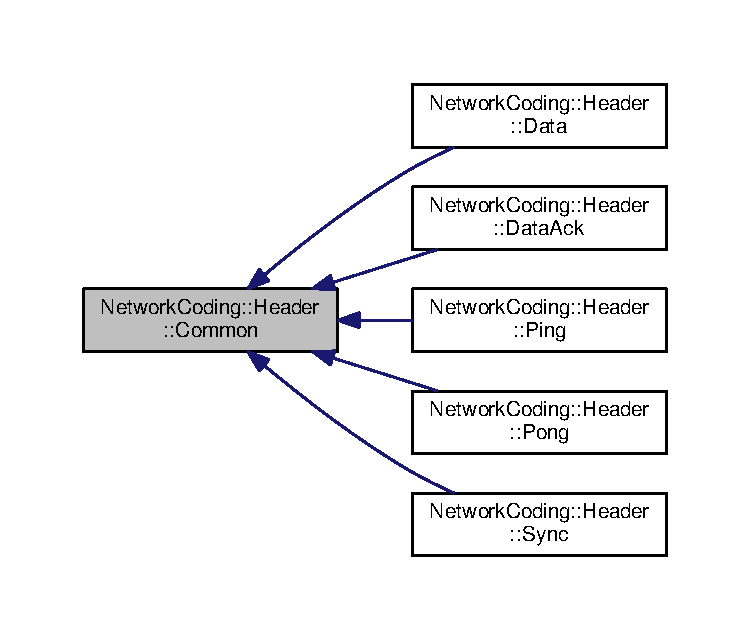
\includegraphics[width=350pt]{struct_network_coding_1_1_header_1_1_common__inherit__graph}
\end{center}
\end{figure}
\subsection*{Public Types}
\begin{DoxyCompactItemize}
\item 
enum {\bfseries Header\+Type} \+: uint8\+\_\+t \{ \\*
{\bfseries D\+A\+TA} = 1, 
{\bfseries S\+Y\+NC}, 
{\bfseries P\+I\+NG}, 
{\bfseries D\+A\+T\+A\+\_\+\+A\+CK}, 
\\*
{\bfseries S\+Y\+N\+C\+\_\+\+A\+CK}, 
{\bfseries P\+O\+NG}
 \}\hypertarget{struct_network_coding_1_1_header_1_1_common_a541c101565c64aee2a50ac90ed9f04b7}{}\label{struct_network_coding_1_1_header_1_1_common_a541c101565c64aee2a50ac90ed9f04b7}

\end{DoxyCompactItemize}
\subsection*{Public Attributes}
\begin{DoxyCompactItemize}
\item 
uint8\+\_\+t {\bfseries m\+\_\+\+Type}\hypertarget{struct_network_coding_1_1_header_1_1_common_a30fe4c3683ca8bb30e98bf75dfce82f3}{}\label{struct_network_coding_1_1_header_1_1_common_a30fe4c3683ca8bb30e98bf75dfce82f3}

\item 
uint8\+\_\+t {\bfseries m\+\_\+\+Check\+Sum}\hypertarget{struct_network_coding_1_1_header_1_1_common_a6e3b1cc0ffc7a903f9fbe1d44eb06d58}{}\label{struct_network_coding_1_1_header_1_1_common_a6e3b1cc0ffc7a903f9fbe1d44eb06d58}

\item 
enum Network\+Coding\+::\+Header\+::\+Common\+::\+Header\+Type {\bfseries \+\_\+\+\_\+attribute\+\_\+\+\_\+}\hypertarget{struct_network_coding_1_1_header_1_1_common_a6b14dbf617e88e01a0d55c8c60ecee40}{}\label{struct_network_coding_1_1_header_1_1_common_a6b14dbf617e88e01a0d55c8c60ecee40}

\end{DoxyCompactItemize}


The documentation for this struct was generated from the following file\+:\begin{DoxyCompactItemize}
\item 
/home/dujeonglee/\+Network\+Coding\+Rev/c\+\_\+cpp/common.\+h\end{DoxyCompactItemize}

\hypertarget{struct_network_coding_1_1_header_1_1_data}{}\section{Network\+Coding\+:\+:Header\+:\+:Data Struct Reference}
\label{struct_network_coding_1_1_header_1_1_data}\index{Network\+Coding\+::\+Header\+::\+Data@{Network\+Coding\+::\+Header\+::\+Data}}


Inheritance diagram for Network\+Coding\+:\+:Header\+:\+:Data\+:\nopagebreak
\begin{figure}[H]
\begin{center}
\leavevmode
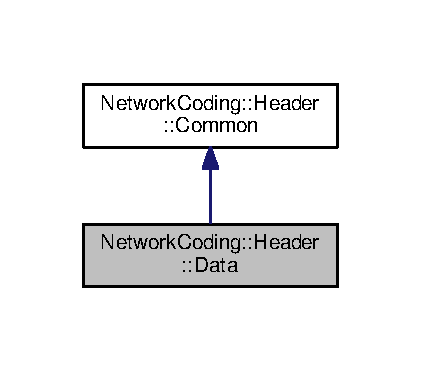
\includegraphics[width=202pt]{struct_network_coding_1_1_header_1_1_data__inherit__graph}
\end{center}
\end{figure}


Collaboration diagram for Network\+Coding\+:\+:Header\+:\+:Data\+:\nopagebreak
\begin{figure}[H]
\begin{center}
\leavevmode
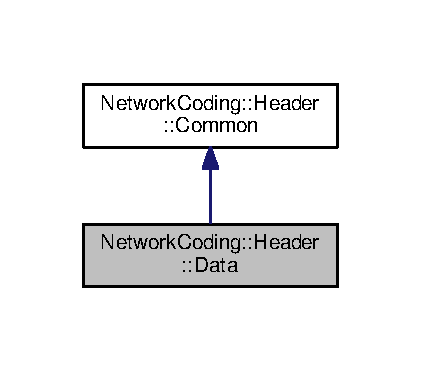
\includegraphics[width=202pt]{struct_network_coding_1_1_header_1_1_data__coll__graph}
\end{center}
\end{figure}
\subsection*{Public Types}
\begin{DoxyCompactItemize}
\item 
enum {\bfseries Data\+Header\+Flag} \+: uint8\+\_\+t \{ {\bfseries F\+L\+A\+G\+S\+\_\+\+O\+R\+I\+G\+I\+N\+AL} = 0x1, 
{\bfseries F\+L\+A\+G\+S\+\_\+\+E\+N\+D\+\_\+\+O\+F\+\_\+\+B\+LK} = 0x2, 
{\bfseries F\+L\+A\+G\+S\+\_\+\+C\+O\+N\+S\+U\+M\+ED} = 0x4
 \}\hypertarget{struct_network_coding_1_1_header_1_1_data_ad108d30572fcdb4464fda2c035910b56}{}\label{struct_network_coding_1_1_header_1_1_data_ad108d30572fcdb4464fda2c035910b56}

\item 
enum {\bfseries Off\+Sets} \+: uint8\+\_\+t \{ {\bfseries Coding\+Offset} = (1 + 1 + 2 + 2 + 2 + 2 + 1 + 1 + 1 + 1)
 \}\hypertarget{struct_network_coding_1_1_header_1_1_data_a5e55347a78baeebc72fb402fd5e30bfc}{}\label{struct_network_coding_1_1_header_1_1_data_a5e55347a78baeebc72fb402fd5e30bfc}

\end{DoxyCompactItemize}
\subsection*{Public Attributes}
\begin{DoxyCompactItemize}
\item 
uint16\+\_\+t {\bfseries m\+\_\+\+Total\+Size}\hypertarget{struct_network_coding_1_1_header_1_1_data_a0eee10996f4c999d5fa17105c376e619}{}\label{struct_network_coding_1_1_header_1_1_data_a0eee10996f4c999d5fa17105c376e619}

\item 
uint16\+\_\+t {\bfseries m\+\_\+\+Min\+Block\+Sequence\+Number}\hypertarget{struct_network_coding_1_1_header_1_1_data_aba45c425ef186557b1707e2071aae988}{}\label{struct_network_coding_1_1_header_1_1_data_aba45c425ef186557b1707e2071aae988}

\item 
uint16\+\_\+t {\bfseries m\+\_\+\+Current\+Block\+Sequence\+Number}\hypertarget{struct_network_coding_1_1_header_1_1_data_a771d12a3f6cf0651e0b89558cd50e4ec}{}\label{struct_network_coding_1_1_header_1_1_data_a771d12a3f6cf0651e0b89558cd50e4ec}

\item 
uint16\+\_\+t {\bfseries m\+\_\+\+Max\+Block\+Sequence\+Number}\hypertarget{struct_network_coding_1_1_header_1_1_data_adaa6e93aa9cf7b836f68d58dcb31ff2f}{}\label{struct_network_coding_1_1_header_1_1_data_adaa6e93aa9cf7b836f68d58dcb31ff2f}

\item 
uint8\+\_\+t {\bfseries m\+\_\+\+Expected\+Rank}\hypertarget{struct_network_coding_1_1_header_1_1_data_aef3bd9133fd1541c8a57bb4398a47685}{}\label{struct_network_coding_1_1_header_1_1_data_aef3bd9133fd1541c8a57bb4398a47685}

\item 
uint8\+\_\+t {\bfseries m\+\_\+\+Maximum\+Rank}\hypertarget{struct_network_coding_1_1_header_1_1_data_a6f01051deb4fadd59c404e76cc1fe186}{}\label{struct_network_coding_1_1_header_1_1_data_a6f01051deb4fadd59c404e76cc1fe186}

\item 
uint8\+\_\+t {\bfseries m\+\_\+\+Flags}\hypertarget{struct_network_coding_1_1_header_1_1_data_adf3d88f0abac9a055403c842249b34d3}{}\label{struct_network_coding_1_1_header_1_1_data_adf3d88f0abac9a055403c842249b34d3}

\item 
uint8\+\_\+t {\bfseries m\+\_\+\+Tx\+Count}\hypertarget{struct_network_coding_1_1_header_1_1_data_ab8f5cc8da3279a862b81ed883ac697cc}{}\label{struct_network_coding_1_1_header_1_1_data_ab8f5cc8da3279a862b81ed883ac697cc}

\item 
uint16\+\_\+t {\bfseries m\+\_\+\+Payload\+Size}\hypertarget{struct_network_coding_1_1_header_1_1_data_a9718b3a6987a63cdca1a1ae09ef79f24}{}\label{struct_network_coding_1_1_header_1_1_data_a9718b3a6987a63cdca1a1ae09ef79f24}

\item 
uint8\+\_\+t \hyperlink{struct_network_coding_1_1_header_1_1_data_a21e3e58d1a143834d9c4490613d3c3ff}{m\+\_\+\+Last\+Indicator}
\item 
uint8\+\_\+t {\bfseries m\+\_\+\+Codes} \mbox{[}1\mbox{]}\hypertarget{struct_network_coding_1_1_header_1_1_data_ae5000aecfcf9559c5cf47c8eea4d8c02}{}\label{struct_network_coding_1_1_header_1_1_data_ae5000aecfcf9559c5cf47c8eea4d8c02}

\end{DoxyCompactItemize}


\subsection{Member Data Documentation}
\index{Network\+Coding\+::\+Header\+::\+Data@{Network\+Coding\+::\+Header\+::\+Data}!m\+\_\+\+Last\+Indicator@{m\+\_\+\+Last\+Indicator}}
\index{m\+\_\+\+Last\+Indicator@{m\+\_\+\+Last\+Indicator}!Network\+Coding\+::\+Header\+::\+Data@{Network\+Coding\+::\+Header\+::\+Data}}
\subsubsection[{\texorpdfstring{m\+\_\+\+Last\+Indicator}{m_LastIndicator}}]{\setlength{\rightskip}{0pt plus 5cm}uint8\+\_\+t Network\+Coding\+::\+Header\+::\+Data\+::m\+\_\+\+Last\+Indicator}\hypertarget{struct_network_coding_1_1_header_1_1_data_a21e3e58d1a143834d9c4490613d3c3ff}{}\label{struct_network_coding_1_1_header_1_1_data_a21e3e58d1a143834d9c4490613d3c3ff}
\begin{DoxyRefDesc}{Todo}
\item[\hyperlink{todo__todo000001}{Todo}]This is reserved for support of fragmentation. \end{DoxyRefDesc}


The documentation for this struct was generated from the following file\+:\begin{DoxyCompactItemize}
\item 
/home/dujeonglee/\+Network\+Coding\+Rev/c\+\_\+cpp/common.\+h\end{DoxyCompactItemize}

\hypertarget{struct_network_coding_1_1_header_1_1_data_ack}{}\section{Network\+Coding\+:\+:Header\+:\+:Data\+Ack Struct Reference}
\label{struct_network_coding_1_1_header_1_1_data_ack}\index{Network\+Coding\+::\+Header\+::\+Data\+Ack@{Network\+Coding\+::\+Header\+::\+Data\+Ack}}


Inheritance diagram for Network\+Coding\+:\+:Header\+:\+:Data\+Ack\+:\nopagebreak
\begin{figure}[H]
\begin{center}
\leavevmode
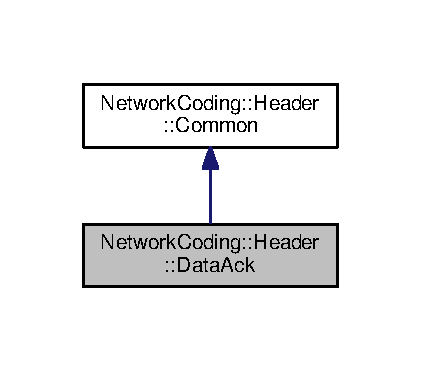
\includegraphics[width=202pt]{struct_network_coding_1_1_header_1_1_data_ack__inherit__graph}
\end{center}
\end{figure}


Collaboration diagram for Network\+Coding\+:\+:Header\+:\+:Data\+Ack\+:\nopagebreak
\begin{figure}[H]
\begin{center}
\leavevmode
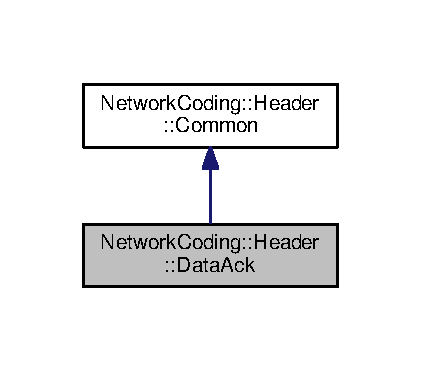
\includegraphics[width=202pt]{struct_network_coding_1_1_header_1_1_data_ack__coll__graph}
\end{center}
\end{figure}
\subsection*{Public Attributes}
\begin{DoxyCompactItemize}
\item 
uint8\+\_\+t {\bfseries m\+\_\+\+Rank}\hypertarget{struct_network_coding_1_1_header_1_1_data_ack_a7b55caf18d0365add6f33ce5c054cee1}{}\label{struct_network_coding_1_1_header_1_1_data_ack_a7b55caf18d0365add6f33ce5c054cee1}

\item 
uint8\+\_\+t {\bfseries m\+\_\+\+Max\+Rank}\hypertarget{struct_network_coding_1_1_header_1_1_data_ack_aa5ed1e395967aa8513ec40f7bbed2769}{}\label{struct_network_coding_1_1_header_1_1_data_ack_aa5ed1e395967aa8513ec40f7bbed2769}

\item 
uint8\+\_\+t {\bfseries m\+\_\+\+Losses}\hypertarget{struct_network_coding_1_1_header_1_1_data_ack_ae10b7d635306ee5a5cb4b48e77a82c9a}{}\label{struct_network_coding_1_1_header_1_1_data_ack_ae10b7d635306ee5a5cb4b48e77a82c9a}

\item 
uint16\+\_\+t {\bfseries m\+\_\+\+Block\+Sequence\+Number}\hypertarget{struct_network_coding_1_1_header_1_1_data_ack_abb7ebded32aa8e1154d09008cdc20d02}{}\label{struct_network_coding_1_1_header_1_1_data_ack_abb7ebded32aa8e1154d09008cdc20d02}

\end{DoxyCompactItemize}
\subsection*{Additional Inherited Members}


The documentation for this struct was generated from the following file\+:\begin{DoxyCompactItemize}
\item 
/home/dujeonglee/\+Network\+Coding\+Rev/c\+\_\+cpp/common.\+h\end{DoxyCompactItemize}

\hypertarget{class_decoding_packet}{}\section{Decoding\+Packet$<$ L\+O\+O\+PS $>$ Class Template Reference}
\label{class_decoding_packet}\index{Decoding\+Packet$<$ L\+O\+O\+P\+S $>$@{Decoding\+Packet$<$ L\+O\+O\+P\+S $>$}}
\subsection*{Static Public Member Functions}
\begin{DoxyCompactItemize}
\item 
static void {\bfseries Run} (std\+::vector$<$ std\+::unique\+\_\+ptr$<$ uint8\+\_\+t\mbox{[}$\,$\mbox{]}$>$$>$ \&out, std\+::vector$<$ std\+::unique\+\_\+ptr$<$ uint8\+\_\+t\mbox{[}$\,$\mbox{]}$>$$>$ \&decoded\+Packet\+Buffer, const std\+::vector$<$ std\+::unique\+\_\+ptr$<$ uint8\+\_\+t\mbox{[}$\,$\mbox{]}$>$$>$ \&decoding\+Matrix, uint32\+\_\+t \&decoding\+Offset, const uint8\+\_\+t decoding\+Index, const uint8\+\_\+t packet\+Index)\hypertarget{class_decoding_packet_afc9daa4ba02b54de271640b2bf368580}{}\label{class_decoding_packet_afc9daa4ba02b54de271640b2bf368580}

\end{DoxyCompactItemize}


The documentation for this class was generated from the following file\+:\begin{DoxyCompactItemize}
\item 
/home/dujeonglee/\+Network\+Coding\+Rev/c\+\_\+cpp/encoding\+\_\+decoding\+\_\+macro.\+h\end{DoxyCompactItemize}

\hypertarget{class_decoding_unrolling}{}\section{Decoding\+Unrolling$<$ L\+O\+O\+PS, I\+T\+ER $>$ Class Template Reference}
\label{class_decoding_unrolling}\index{Decoding\+Unrolling$<$ L\+O\+O\+P\+S, I\+T\+E\+R $>$@{Decoding\+Unrolling$<$ L\+O\+O\+P\+S, I\+T\+E\+R $>$}}
\subsection*{Static Public Member Functions}
\begin{DoxyCompactItemize}
\item 
static void {\bfseries Run} (std\+::vector$<$ std\+::unique\+\_\+ptr$<$ uint8\+\_\+t\mbox{[}$\,$\mbox{]}$>$$>$ \&out, std\+::vector$<$ std\+::unique\+\_\+ptr$<$ uint8\+\_\+t\mbox{[}$\,$\mbox{]}$>$$>$ \&decoded\+Packet\+Buffer, const std\+::vector$<$ std\+::unique\+\_\+ptr$<$ uint8\+\_\+t\mbox{[}$\,$\mbox{]}$>$$>$ \&decoding\+Matrix, uint32\+\_\+t \&decoding\+Offset, const uint8\+\_\+t decoding\+Index, const uint8\+\_\+t packet\+Index)\hypertarget{class_decoding_unrolling_a5ece7fc8d2bcb999ad56e39caaf702bb}{}\label{class_decoding_unrolling_a5ece7fc8d2bcb999ad56e39caaf702bb}

\end{DoxyCompactItemize}


The documentation for this class was generated from the following file\+:\begin{DoxyCompactItemize}
\item 
/home/dujeonglee/\+Network\+Coding\+Rev/c\+\_\+cpp/encoding\+\_\+decoding\+\_\+macro.\+h\end{DoxyCompactItemize}

\hypertarget{class_decoding_unrolling_3_01_l_o_o_p_s_00_01_l_o_o_p_s_01_4}{}\section{Decoding\+Unrolling$<$ L\+O\+O\+PS, L\+O\+O\+PS $>$ Class Template Reference}
\label{class_decoding_unrolling_3_01_l_o_o_p_s_00_01_l_o_o_p_s_01_4}\index{Decoding\+Unrolling$<$ L\+O\+O\+P\+S, L\+O\+O\+P\+S $>$@{Decoding\+Unrolling$<$ L\+O\+O\+P\+S, L\+O\+O\+P\+S $>$}}
\subsection*{Static Public Member Functions}
\begin{DoxyCompactItemize}
\item 
static void {\bfseries Run} (std\+::vector$<$ std\+::unique\+\_\+ptr$<$ uint8\+\_\+t\mbox{[}$\,$\mbox{]}$>$$>$ \&out, std\+::vector$<$ std\+::unique\+\_\+ptr$<$ uint8\+\_\+t\mbox{[}$\,$\mbox{]}$>$$>$ \&decoded\+Packet\+Buffer, const std\+::vector$<$ std\+::unique\+\_\+ptr$<$ uint8\+\_\+t\mbox{[}$\,$\mbox{]}$>$$>$ \&decoding\+Matrix, uint32\+\_\+t \&decoding\+Offset, const uint8\+\_\+t decoding\+Index, const uint8\+\_\+t packet\+Index)\hypertarget{class_decoding_unrolling_3_01_l_o_o_p_s_00_01_l_o_o_p_s_01_4_addb067d41781dd919d9a1735a4744e24}{}\label{class_decoding_unrolling_3_01_l_o_o_p_s_00_01_l_o_o_p_s_01_4_addb067d41781dd919d9a1735a4744e24}

\end{DoxyCompactItemize}


The documentation for this class was generated from the following file\+:\begin{DoxyCompactItemize}
\item 
/home/dujeonglee/\+Network\+Coding\+Rev/c\+\_\+cpp/encoding\+\_\+decoding\+\_\+macro.\+h\end{DoxyCompactItemize}

\hypertarget{class_encoding_packet}{}\section{Encoding\+Packet$<$ L\+O\+O\+PS $>$ Class Template Reference}
\label{class_encoding_packet}\index{Encoding\+Packet$<$ L\+O\+O\+P\+S $>$@{Encoding\+Packet$<$ L\+O\+O\+P\+S $>$}}
\subsection*{Static Public Member Functions}
\begin{DoxyCompactItemize}
\item 
static void {\bfseries Run} (uint8\+\_\+t $\ast$remedy\+Packet\+Buffer, uint8\+\_\+t $\ast$original\+Packet\+Buffer, const std\+::vector$<$ uint8\+\_\+t $>$ \&random\+Coefficients, uint16\+\_\+t \&coding\+Offset, const uint8\+\_\+t packet\+Index)\hypertarget{class_encoding_packet_a543e673d0afa8141ec064877e99d71c9}{}\label{class_encoding_packet_a543e673d0afa8141ec064877e99d71c9}

\end{DoxyCompactItemize}


The documentation for this class was generated from the following file\+:\begin{DoxyCompactItemize}
\item 
/home/dujeonglee/\+Network\+Coding\+Rev/c\+\_\+cpp/encoding\+\_\+decoding\+\_\+macro.\+h\end{DoxyCompactItemize}

\hypertarget{class_encoding_unrolling}{}\section{Encoding\+Unrolling$<$ L\+O\+O\+PS, I\+T\+ER $>$ Class Template Reference}
\label{class_encoding_unrolling}\index{Encoding\+Unrolling$<$ L\+O\+O\+P\+S, I\+T\+E\+R $>$@{Encoding\+Unrolling$<$ L\+O\+O\+P\+S, I\+T\+E\+R $>$}}
\subsection*{Static Public Member Functions}
\begin{DoxyCompactItemize}
\item 
static void {\bfseries Run} (uint8\+\_\+t $\ast$remedy\+Packet\+Buffer, uint8\+\_\+t $\ast$original\+Packet\+Buffer, const std\+::vector$<$ uint8\+\_\+t $>$ \&random\+Coefficients, uint16\+\_\+t \&coding\+Offset, const uint8\+\_\+t packet\+Index)\hypertarget{class_encoding_unrolling_a7c36b3fced839de91e82a14ae480bec4}{}\label{class_encoding_unrolling_a7c36b3fced839de91e82a14ae480bec4}

\end{DoxyCompactItemize}


The documentation for this class was generated from the following file\+:\begin{DoxyCompactItemize}
\item 
/home/dujeonglee/\+Network\+Coding\+Rev/c\+\_\+cpp/encoding\+\_\+decoding\+\_\+macro.\+h\end{DoxyCompactItemize}

\hypertarget{class_encoding_unrolling_3_01_l_o_o_p_s_00_01_l_o_o_p_s_01_4}{}\section{Encoding\+Unrolling$<$ L\+O\+O\+PS, L\+O\+O\+PS $>$ Class Template Reference}
\label{class_encoding_unrolling_3_01_l_o_o_p_s_00_01_l_o_o_p_s_01_4}\index{Encoding\+Unrolling$<$ L\+O\+O\+P\+S, L\+O\+O\+P\+S $>$@{Encoding\+Unrolling$<$ L\+O\+O\+P\+S, L\+O\+O\+P\+S $>$}}
\subsection*{Static Public Member Functions}
\begin{DoxyCompactItemize}
\item 
static void {\bfseries Run} (uint8\+\_\+t $\ast$remedy\+Packet\+Buffer, uint8\+\_\+t $\ast$original\+Packet\+Buffer, const std\+::vector$<$ uint8\+\_\+t $>$ \&random\+Coefficients, uint16\+\_\+t \&coding\+Offset, const uint8\+\_\+t packet\+Index)\hypertarget{class_encoding_unrolling_3_01_l_o_o_p_s_00_01_l_o_o_p_s_01_4_a8f388974b4b556d2bf89680c21739316}{}\label{class_encoding_unrolling_3_01_l_o_o_p_s_00_01_l_o_o_p_s_01_4_a8f388974b4b556d2bf89680c21739316}

\end{DoxyCompactItemize}


The documentation for this class was generated from the following file\+:\begin{DoxyCompactItemize}
\item 
/home/dujeonglee/\+Network\+Coding\+Rev/c\+\_\+cpp/encoding\+\_\+decoding\+\_\+macro.\+h\end{DoxyCompactItemize}

\hypertarget{class_network_coding_1_1_finite_field}{}\section{Network\+Coding\+:\+:Finite\+Field Class Reference}
\label{class_network_coding_1_1_finite_field}\index{Network\+Coding\+::\+Finite\+Field@{Network\+Coding\+::\+Finite\+Field}}
\subsection*{Public Member Functions}
\begin{DoxyCompactItemize}
\item 
byte \hyperlink{class_network_coding_1_1_finite_field_ad5d01d29f41b81e04c2c38774d46f9df}{add} (byte a, byte b)\hypertarget{class_network_coding_1_1_finite_field_ad5d01d29f41b81e04c2c38774d46f9df}{}\label{class_network_coding_1_1_finite_field_ad5d01d29f41b81e04c2c38774d46f9df}

\begin{DoxyCompactList}\small\item\em add\+: Adding \char`\"{}a\char`\"{} and \char`\"{}b\char`\"{} \end{DoxyCompactList}\item 
byte \hyperlink{class_network_coding_1_1_finite_field_a4ab96138860cf53a2b2958f425e9702d}{sub} (byte a, byte b)\hypertarget{class_network_coding_1_1_finite_field_a4ab96138860cf53a2b2958f425e9702d}{}\label{class_network_coding_1_1_finite_field_a4ab96138860cf53a2b2958f425e9702d}

\begin{DoxyCompactList}\small\item\em sub\+: Subtracting \char`\"{}b\char`\"{} from \char`\"{}a\char`\"{} \end{DoxyCompactList}\item 
byte \hyperlink{class_network_coding_1_1_finite_field_affb07a8a5bb0d0d46d8e4ddd15e6eb71}{mul} (byte a, byte b)\hypertarget{class_network_coding_1_1_finite_field_affb07a8a5bb0d0d46d8e4ddd15e6eb71}{}\label{class_network_coding_1_1_finite_field_affb07a8a5bb0d0d46d8e4ddd15e6eb71}

\begin{DoxyCompactList}\small\item\em mul\+: Multiplying \char`\"{}a\char`\"{} and \char`\"{}b\char`\"{} \end{DoxyCompactList}\item 
byte \hyperlink{class_network_coding_1_1_finite_field_a9bc9e49525ea45553459fcee844325c7}{inv} (byte a)\hypertarget{class_network_coding_1_1_finite_field_a9bc9e49525ea45553459fcee844325c7}{}\label{class_network_coding_1_1_finite_field_a9bc9e49525ea45553459fcee844325c7}

\begin{DoxyCompactList}\small\item\em inv\+: Calculating inverse of \char`\"{}a\char`\"{} \end{DoxyCompactList}\end{DoxyCompactItemize}
\subsection*{Static Public Member Functions}
\begin{DoxyCompactItemize}
\item 
static \hyperlink{class_network_coding_1_1_finite_field}{Finite\+Field} $\ast$ {\bfseries instance} ()\hypertarget{class_network_coding_1_1_finite_field_a427c30d3fd41550434292c36ce88a8dc}{}\label{class_network_coding_1_1_finite_field_a427c30d3fd41550434292c36ce88a8dc}

\end{DoxyCompactItemize}


The documentation for this class was generated from the following files\+:\begin{DoxyCompactItemize}
\item 
/home/dujeonglee/\+Network\+Coding\+Rev/c\+\_\+cpp/finite\+\_\+field.\+h\item 
/home/dujeonglee/\+Network\+Coding\+Rev/c\+\_\+cpp/finite\+\_\+field.\+cpp\end{DoxyCompactItemize}

\hypertarget{class_network_coding_1_1_n_c_socket}{}\section{Network\+Coding\+:\+:N\+C\+Socket Class Reference}
\label{class_network_coding_1_1_n_c_socket}\index{Network\+Coding\+::\+N\+C\+Socket@{Network\+Coding\+::\+N\+C\+Socket}}
\subsection*{Public Member Functions}
\begin{DoxyCompactItemize}
\item 
{\bfseries N\+C\+Socket} (const \hyperlink{class_network_coding_1_1_n_c_socket}{N\+C\+Socket} \&)=delete\hypertarget{class_network_coding_1_1_n_c_socket_a23e2cac75f11b839938b2acbaf3acaa7}{}\label{class_network_coding_1_1_n_c_socket_a23e2cac75f11b839938b2acbaf3acaa7}

\item 
{\bfseries N\+C\+Socket} (\hyperlink{class_network_coding_1_1_n_c_socket}{N\+C\+Socket} \&\&)=delete\hypertarget{class_network_coding_1_1_n_c_socket_a135586fbe7ba03e08a258172bf32bd44}{}\label{class_network_coding_1_1_n_c_socket_a135586fbe7ba03e08a258172bf32bd44}

\item 
{\bfseries N\+C\+Socket} (const std\+::string P\+O\+RT, const uint32\+\_\+t R\+X\+T\+I\+M\+E\+O\+UT, const uint32\+\_\+t T\+X\+T\+I\+M\+E\+O\+UT, const std\+::function$<$ void(uint8\+\_\+t $\ast$const buffer, const uint16\+\_\+t length, const sockaddr $\ast$const sender\+\_\+addr, const uint32\+\_\+t sender\+\_\+addr\+\_\+len)$>$ rx)\hypertarget{class_network_coding_1_1_n_c_socket_acf1ee3b4bebbe25a6dd6dfdee9b1fdfb}{}\label{class_network_coding_1_1_n_c_socket_acf1ee3b4bebbe25a6dd6dfdee9b1fdfb}

\item 
\hyperlink{class_network_coding_1_1_n_c_socket}{N\+C\+Socket} \& {\bfseries operator=} (const \hyperlink{class_network_coding_1_1_n_c_socket}{N\+C\+Socket} \&)=delete\hypertarget{class_network_coding_1_1_n_c_socket_a440c01c767596edc5dab1bc9f80824f3}{}\label{class_network_coding_1_1_n_c_socket_a440c01c767596edc5dab1bc9f80824f3}

\item 
\hyperlink{class_network_coding_1_1_n_c_socket}{N\+C\+Socket} \& {\bfseries operator=} (\hyperlink{class_network_coding_1_1_n_c_socket}{N\+C\+Socket} \&\&)=delete\hypertarget{class_network_coding_1_1_n_c_socket_ab8ca12964a95b2a54d86a7b4e6325ca9}{}\label{class_network_coding_1_1_n_c_socket_ab8ca12964a95b2a54d86a7b4e6325ca9}

\item 
bool {\bfseries Connect} (const std\+::string ip, const std\+::string port, const uint32\+\_\+t timeout, const Parameter\+::\+T\+R\+A\+N\+S\+M\+I\+S\+S\+I\+O\+N\+\_\+\+M\+O\+DE Transmission\+Mode, const Parameter\+::\+B\+L\+O\+C\+K\+\_\+\+S\+I\+ZE Block\+Size, const uint16\+\_\+t Retransmission\+Redundancy)\hypertarget{class_network_coding_1_1_n_c_socket_a1374c825f9a5403fbccf48b55ba051fd}{}\label{class_network_coding_1_1_n_c_socket_a1374c825f9a5403fbccf48b55ba051fd}

\item 
void {\bfseries Disconnect} (const std\+::string ip, const std\+::string port)\hypertarget{class_network_coding_1_1_n_c_socket_a96394c488e1f394c624202c85a60e9e0}{}\label{class_network_coding_1_1_n_c_socket_a96394c488e1f394c624202c85a60e9e0}

\item 
bool {\bfseries Send} (const std\+::string ip, const std\+::string port, uint8\+\_\+t $\ast$const buff, const uint16\+\_\+t size)\hypertarget{class_network_coding_1_1_n_c_socket_a68d0a54287a8ccaad0635cac3e24d8b2}{}\label{class_network_coding_1_1_n_c_socket_a68d0a54287a8ccaad0635cac3e24d8b2}

\item 
bool {\bfseries Flush} (const std\+::string ip, const std\+::string port)\hypertarget{class_network_coding_1_1_n_c_socket_a2a507dbb11c5c85c1604c45466f2ae87}{}\label{class_network_coding_1_1_n_c_socket_a2a507dbb11c5c85c1604c45466f2ae87}

\item 
void {\bfseries Wait\+Until\+Tx\+Is\+Completed} (const std\+::string ip, const std\+::string port)\hypertarget{class_network_coding_1_1_n_c_socket_ac7d30bf07839598f790e702766e720cd}{}\label{class_network_coding_1_1_n_c_socket_ac7d30bf07839598f790e702766e720cd}

\item 
bool {\bfseries Receive} (uint8\+\_\+t $\ast$const buffer, uint16\+\_\+t $\ast$const length, sockaddr $\ast$const sender\+\_\+addr, uint32\+\_\+t $\ast$const sender\+\_\+addr\+\_\+len, uint32\+\_\+t timeout)\hypertarget{class_network_coding_1_1_n_c_socket_afb8b2cf0fa29cd712f4cee4edc6d71b8}{}\label{class_network_coding_1_1_n_c_socket_afb8b2cf0fa29cd712f4cee4edc6d71b8}

\end{DoxyCompactItemize}


The documentation for this class was generated from the following file\+:\begin{DoxyCompactItemize}
\item 
/home/dujeonglee/\+Network\+Coding\+Rev/c\+\_\+cpp/ncsocket.\+h\end{DoxyCompactItemize}

\hypertarget{struct_network_coding_1_1_header_1_1_ping}{}\section{Network\+Coding\+:\+:Header\+:\+:Ping Struct Reference}
\label{struct_network_coding_1_1_header_1_1_ping}\index{Network\+Coding\+::\+Header\+::\+Ping@{Network\+Coding\+::\+Header\+::\+Ping}}


Inheritance diagram for Network\+Coding\+:\+:Header\+:\+:Ping\+:\nopagebreak
\begin{figure}[H]
\begin{center}
\leavevmode
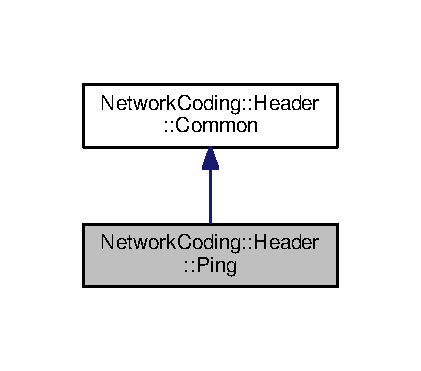
\includegraphics[width=202pt]{struct_network_coding_1_1_header_1_1_ping__inherit__graph}
\end{center}
\end{figure}


Collaboration diagram for Network\+Coding\+:\+:Header\+:\+:Ping\+:\nopagebreak
\begin{figure}[H]
\begin{center}
\leavevmode
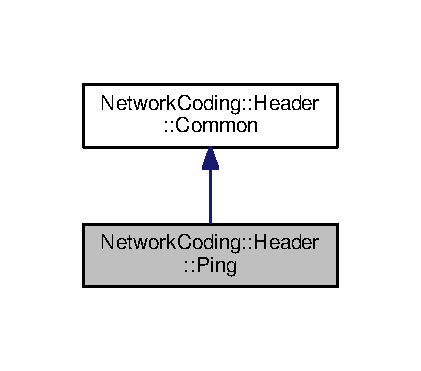
\includegraphics[width=202pt]{struct_network_coding_1_1_header_1_1_ping__coll__graph}
\end{center}
\end{figure}
\subsection*{Public Attributes}
\begin{DoxyCompactItemize}
\item 
C\+L\+O\+C\+K\+::time\+\_\+point\+::duration\+::rep {\bfseries m\+\_\+\+Ping\+Time}\hypertarget{struct_network_coding_1_1_header_1_1_ping_adf48346b5f6f3438534c14943b72a098}{}\label{struct_network_coding_1_1_header_1_1_ping_adf48346b5f6f3438534c14943b72a098}

\end{DoxyCompactItemize}
\subsection*{Additional Inherited Members}


The documentation for this struct was generated from the following file\+:\begin{DoxyCompactItemize}
\item 
/home/dujeonglee/\+Network\+Coding\+Rev/c\+\_\+cpp/common.\+h\end{DoxyCompactItemize}

\hypertarget{struct_network_coding_1_1_header_1_1_pong}{}\section{Network\+Coding\+:\+:Header\+:\+:Pong Struct Reference}
\label{struct_network_coding_1_1_header_1_1_pong}\index{Network\+Coding\+::\+Header\+::\+Pong@{Network\+Coding\+::\+Header\+::\+Pong}}


Inheritance diagram for Network\+Coding\+:\+:Header\+:\+:Pong\+:\nopagebreak
\begin{figure}[H]
\begin{center}
\leavevmode
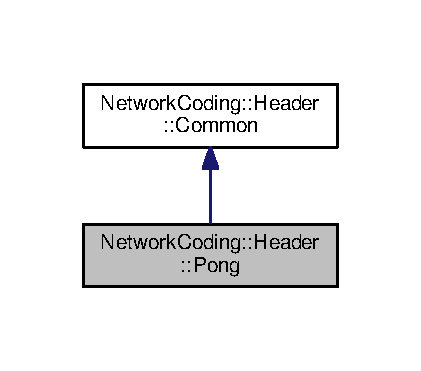
\includegraphics[width=202pt]{struct_network_coding_1_1_header_1_1_pong__inherit__graph}
\end{center}
\end{figure}


Collaboration diagram for Network\+Coding\+:\+:Header\+:\+:Pong\+:\nopagebreak
\begin{figure}[H]
\begin{center}
\leavevmode
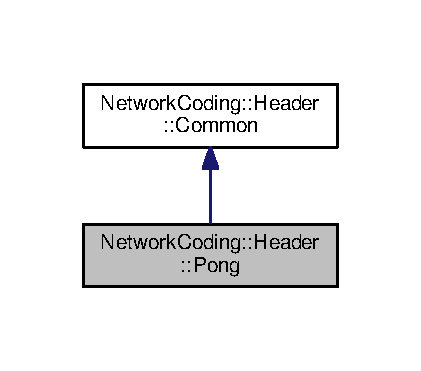
\includegraphics[width=202pt]{struct_network_coding_1_1_header_1_1_pong__coll__graph}
\end{center}
\end{figure}
\subsection*{Public Attributes}
\begin{DoxyCompactItemize}
\item 
C\+L\+O\+C\+K\+::time\+\_\+point\+::duration\+::rep {\bfseries m\+\_\+\+Ping\+Time}\hypertarget{struct_network_coding_1_1_header_1_1_pong_adf16054eedcffdd9c09bec8449493b67}{}\label{struct_network_coding_1_1_header_1_1_pong_adf16054eedcffdd9c09bec8449493b67}

\end{DoxyCompactItemize}
\subsection*{Additional Inherited Members}


The documentation for this struct was generated from the following file\+:\begin{DoxyCompactItemize}
\item 
/home/dujeonglee/\+Network\+Coding\+Rev/c\+\_\+cpp/common.\+h\end{DoxyCompactItemize}

\hypertarget{class_network_coding_1_1_reception}{}\section{Network\+Coding\+:\+:Reception Class Reference}
\label{class_network_coding_1_1_reception}\index{Network\+Coding\+::\+Reception@{Network\+Coding\+::\+Reception}}
\subsection*{Public Member Functions}
\begin{DoxyCompactItemize}
\item 
{\bfseries Reception} (const int32\+\_\+t Socket, const std\+::function$<$ void(uint8\+\_\+t $\ast$buffer, uint16\+\_\+t length, const sockaddr $\ast$const sender\+\_\+addr, const uint32\+\_\+t sender\+\_\+addr\+\_\+len)$>$ rx)\hypertarget{class_network_coding_1_1_reception_a217e7e7924e2f8d7d0e93c95eb7802d0}{}\label{class_network_coding_1_1_reception_a217e7e7924e2f8d7d0e93c95eb7802d0}

\item 
void {\bfseries Rx\+Handler} (uint8\+\_\+t $\ast$const buffer, const uint16\+\_\+t size, const sockaddr $\ast$const sender\+\_\+addr, const uint32\+\_\+t sender\+\_\+addr\+\_\+len)\hypertarget{class_network_coding_1_1_reception_ad726803ebdc2d2761e0e11f6affcd488}{}\label{class_network_coding_1_1_reception_ad726803ebdc2d2761e0e11f6affcd488}

\item 
bool {\bfseries Receive} (uint8\+\_\+t $\ast$const buffer, uint16\+\_\+t $\ast$const length, sockaddr $\ast$const sender\+\_\+addr, uint32\+\_\+t $\ast$const sender\+\_\+addr\+\_\+len, uint32\+\_\+t timeout)\hypertarget{class_network_coding_1_1_reception_a1b1a8112382aeb967f46b73e385954d7}{}\label{class_network_coding_1_1_reception_a1b1a8112382aeb967f46b73e385954d7}

\end{DoxyCompactItemize}
\subsection*{Public Attributes}
\begin{DoxyCompactItemize}
\item 
const std\+::function$<$ void(uint8\+\_\+t $\ast$const buffer, const uint16\+\_\+t length, const sockaddr $\ast$const sender\+\_\+addr, const uint32\+\_\+t sender\+\_\+addr\+\_\+len)$>$ {\bfseries m\+\_\+\+Rx\+Callback}\hypertarget{class_network_coding_1_1_reception_af4982d41ddad866f366f7d17a29c7de0}{}\label{class_network_coding_1_1_reception_af4982d41ddad866f366f7d17a29c7de0}

\item 
std\+::mutex {\bfseries m\+\_\+\+Packet\+Queue\+Lock}\hypertarget{class_network_coding_1_1_reception_a49d297f20d3c70cc334ff76846d912d4}{}\label{class_network_coding_1_1_reception_a49d297f20d3c70cc334ff76846d912d4}

\item 
std\+::condition\+\_\+variable {\bfseries m\+\_\+\+Condition}\hypertarget{class_network_coding_1_1_reception_ad79660bdfc37f6d0f1c5d91059ba0c8e}{}\label{class_network_coding_1_1_reception_ad79660bdfc37f6d0f1c5d91059ba0c8e}

\item 
std\+::deque$<$ std\+::tuple$<$ \hyperlink{class_network_coding_1_1_data_types_1_1_address}{Data\+Types\+::\+Address}, uint8\+\_\+t $\ast$ $>$ $>$ {\bfseries m\+\_\+\+Packet\+Queue}\hypertarget{class_network_coding_1_1_reception_adc73afa8de48a266ff81eef3a023e3b4}{}\label{class_network_coding_1_1_reception_adc73afa8de48a266ff81eef3a023e3b4}

\end{DoxyCompactItemize}
\subsection*{Friends}
\begin{DoxyCompactItemize}
\item 
class {\bfseries Reception\+Block}\hypertarget{class_network_coding_1_1_reception_a3b0db9f68934c426ad673e63d3183b29}{}\label{class_network_coding_1_1_reception_a3b0db9f68934c426ad673e63d3183b29}

\item 
class {\bfseries Reception\+Session}\hypertarget{class_network_coding_1_1_reception_a6ed072e1f429e5e4bda0467d37cf64b8}{}\label{class_network_coding_1_1_reception_a6ed072e1f429e5e4bda0467d37cf64b8}

\end{DoxyCompactItemize}


The documentation for this class was generated from the following files\+:\begin{DoxyCompactItemize}
\item 
/home/dujeonglee/\+Network\+Coding\+Rev/c\+\_\+cpp/rx.\+h\item 
/home/dujeonglee/\+Network\+Coding\+Rev/c\+\_\+cpp/rx.\+cpp\end{DoxyCompactItemize}

\hypertarget{class_network_coding_1_1_reception_block}{}\section{Network\+Coding\+:\+:Reception\+Block Class Reference}
\label{class_network_coding_1_1_reception_block}\index{Network\+Coding\+::\+Reception\+Block@{Network\+Coding\+::\+Reception\+Block}}
\subsection*{Public Member Functions}
\begin{DoxyCompactItemize}
\item 
{\bfseries Reception\+Block} (const \hyperlink{class_network_coding_1_1_reception_block}{Reception\+Block} \&)=delete\hypertarget{class_network_coding_1_1_reception_block_ab2ddf47c1360c4551a204480c33b4ad1}{}\label{class_network_coding_1_1_reception_block_ab2ddf47c1360c4551a204480c33b4ad1}

\item 
{\bfseries Reception\+Block} (\hyperlink{class_network_coding_1_1_reception_block}{Reception\+Block} \&\&)=delete\hypertarget{class_network_coding_1_1_reception_block_a626c34996888a2fb98c52d64938ac60c}{}\label{class_network_coding_1_1_reception_block_a626c34996888a2fb98c52d64938ac60c}

\item 
\hyperlink{class_network_coding_1_1_reception_block}{Reception\+Block} \& {\bfseries operator=} (const \hyperlink{class_network_coding_1_1_reception_block}{Reception\+Block} \&)=delete\hypertarget{class_network_coding_1_1_reception_block_a678b299cebefbc366fcce9cca3f2cd45}{}\label{class_network_coding_1_1_reception_block_a678b299cebefbc366fcce9cca3f2cd45}

\item 
\hyperlink{class_network_coding_1_1_reception_block}{Reception\+Block} \& {\bfseries operator=} (\hyperlink{class_network_coding_1_1_reception_block}{Reception\+Block} \&\&)=delete\hypertarget{class_network_coding_1_1_reception_block_a0c0b09d88ce90b3d8dcbb45609c63d11}{}\label{class_network_coding_1_1_reception_block_a0c0b09d88ce90b3d8dcbb45609c63d11}

\item 
{\bfseries Reception\+Block} (\hyperlink{class_network_coding_1_1_reception}{Reception} $\ast$const reception, \hyperlink{class_network_coding_1_1_reception_session}{Reception\+Session} $\ast$const session, const uint16\+\_\+t Block\+Sequence\+Number)\hypertarget{class_network_coding_1_1_reception_block_a3d597dff980e67ef390814aa68dc4c34}{}\label{class_network_coding_1_1_reception_block_a3d597dff980e67ef390814aa68dc4c34}

\item 
void {\bfseries Receive} (uint8\+\_\+t $\ast$const buffer, const uint16\+\_\+t length, const sockaddr $\ast$const sender\+\_\+addr, const uint32\+\_\+t sender\+\_\+addr\+\_\+len)\hypertarget{class_network_coding_1_1_reception_block_a2a316e074d767a80fdf7838b372d4bca}{}\label{class_network_coding_1_1_reception_block_a2a316e074d767a80fdf7838b372d4bca}

\end{DoxyCompactItemize}
\subsection*{Friends}
\begin{DoxyCompactItemize}
\item 
class {\bfseries Reception\+Session}\hypertarget{class_network_coding_1_1_reception_block_a6ed072e1f429e5e4bda0467d37cf64b8}{}\label{class_network_coding_1_1_reception_block_a6ed072e1f429e5e4bda0467d37cf64b8}

\item 
class {\bfseries Reception}\hypertarget{class_network_coding_1_1_reception_block_ab65c4855c6a2c2d0c0b90c5108518547}{}\label{class_network_coding_1_1_reception_block_ab65c4855c6a2c2d0c0b90c5108518547}

\end{DoxyCompactItemize}


The documentation for this class was generated from the following files\+:\begin{DoxyCompactItemize}
\item 
/home/dujeonglee/\+Network\+Coding\+Rev/c\+\_\+cpp/rx.\+h\item 
/home/dujeonglee/\+Network\+Coding\+Rev/c\+\_\+cpp/rx.\+cpp\end{DoxyCompactItemize}

\hypertarget{class_network_coding_1_1_reception_session}{}\section{Network\+Coding\+:\+:Reception\+Session Class Reference}
\label{class_network_coding_1_1_reception_session}\index{Network\+Coding\+::\+Reception\+Session@{Network\+Coding\+::\+Reception\+Session}}
\subsection*{Public Member Functions}
\begin{DoxyCompactItemize}
\item 
{\bfseries Reception\+Session} (const \hyperlink{class_network_coding_1_1_reception_session}{Reception\+Session} \&)=delete\hypertarget{class_network_coding_1_1_reception_session_a4dd8055cd68c112e013961467b65d8f1}{}\label{class_network_coding_1_1_reception_session_a4dd8055cd68c112e013961467b65d8f1}

\item 
{\bfseries Reception\+Session} (\hyperlink{class_network_coding_1_1_reception_session}{Reception\+Session} \&\&)=delete\hypertarget{class_network_coding_1_1_reception_session_a8dbf8ae62db0e6264d5e5a39f795134c}{}\label{class_network_coding_1_1_reception_session_a8dbf8ae62db0e6264d5e5a39f795134c}

\item 
\hyperlink{class_network_coding_1_1_reception_session}{Reception\+Session} \& {\bfseries operator=} (const \hyperlink{class_network_coding_1_1_reception_session}{Reception\+Session} \&)=delete\hypertarget{class_network_coding_1_1_reception_session_a2f00293304a98eafcb58fa87758184c0}{}\label{class_network_coding_1_1_reception_session_a2f00293304a98eafcb58fa87758184c0}

\item 
\hyperlink{class_network_coding_1_1_reception_session}{Reception\+Session} \& {\bfseries operator=} (\hyperlink{class_network_coding_1_1_reception_session}{Reception\+Session} \&\&)=delete\hypertarget{class_network_coding_1_1_reception_session_a7ed969988ed2291db12ccc5c2be791d8}{}\label{class_network_coding_1_1_reception_session_a7ed969988ed2291db12ccc5c2be791d8}

\item 
{\bfseries Reception\+Session} (\hyperlink{class_network_coding_1_1_reception}{Reception} $\ast$const Session, const \hyperlink{class_network_coding_1_1_data_types_1_1_address}{Data\+Types\+::\+Address} addr)\hypertarget{class_network_coding_1_1_reception_session_a704be31ca772fe0e7752715ac6f50cce}{}\label{class_network_coding_1_1_reception_session_a704be31ca772fe0e7752715ac6f50cce}

\item 
void {\bfseries Send\+Data\+Ack} (const \hyperlink{struct_network_coding_1_1_header_1_1_data}{Header\+::\+Data} $\ast$const header, const sockaddr $\ast$const sender\+\_\+addr, const uint32\+\_\+t sender\+\_\+addr\+\_\+len, const uint8\+\_\+t completed=1)\hypertarget{class_network_coding_1_1_reception_session_a77e5e682b295c7dd449b75530494830e}{}\label{class_network_coding_1_1_reception_session_a77e5e682b295c7dd449b75530494830e}

\item 
void {\bfseries Receive} (uint8\+\_\+t $\ast$const buffer, const uint16\+\_\+t length, const sockaddr $\ast$const sender\+\_\+addr, const uint32\+\_\+t sender\+\_\+addr\+\_\+len)\hypertarget{class_network_coding_1_1_reception_session_a526ea619f4713827cfc481f8b25a44ba}{}\label{class_network_coding_1_1_reception_session_a526ea619f4713827cfc481f8b25a44ba}

\end{DoxyCompactItemize}
\subsection*{Friends}
\begin{DoxyCompactItemize}
\item 
class {\bfseries Reception\+Block}\hypertarget{class_network_coding_1_1_reception_session_a3b0db9f68934c426ad673e63d3183b29}{}\label{class_network_coding_1_1_reception_session_a3b0db9f68934c426ad673e63d3183b29}

\item 
class {\bfseries Reception}\hypertarget{class_network_coding_1_1_reception_session_ab65c4855c6a2c2d0c0b90c5108518547}{}\label{class_network_coding_1_1_reception_session_ab65c4855c6a2c2d0c0b90c5108518547}

\end{DoxyCompactItemize}


The documentation for this class was generated from the following files\+:\begin{DoxyCompactItemize}
\item 
/home/dujeonglee/\+Network\+Coding\+Rev/c\+\_\+cpp/rx.\+h\item 
/home/dujeonglee/\+Network\+Coding\+Rev/c\+\_\+cpp/rx.\+cpp\end{DoxyCompactItemize}

\hypertarget{class_network_coding_1_1_data_types_1_1_session_key}{}\section{Network\+Coding\+:\+:Data\+Types\+:\+:Session\+Key Class Reference}
\label{class_network_coding_1_1_data_types_1_1_session_key}\index{Network\+Coding\+::\+Data\+Types\+::\+Session\+Key@{Network\+Coding\+::\+Data\+Types\+::\+Session\+Key}}
\subsection*{Public Attributes}
\begin{DoxyCompactItemize}
\item 
uint64\+\_\+t {\bfseries m\+\_\+\+E\+UI}\hypertarget{class_network_coding_1_1_data_types_1_1_session_key_a302ca92409a4c037326fb1d7c0f71041}{}\label{class_network_coding_1_1_data_types_1_1_session_key_a302ca92409a4c037326fb1d7c0f71041}

\item 
uint16\+\_\+t {\bfseries m\+\_\+\+Port}\hypertarget{class_network_coding_1_1_data_types_1_1_session_key_a954eb8e0e38dc38180a535be0bb17b2a}{}\label{class_network_coding_1_1_data_types_1_1_session_key_a954eb8e0e38dc38180a535be0bb17b2a}

\end{DoxyCompactItemize}


The documentation for this class was generated from the following file\+:\begin{DoxyCompactItemize}
\item 
/home/dujeonglee/\+Network\+Coding\+Rev/c\+\_\+cpp/common.\+h\end{DoxyCompactItemize}

\hypertarget{struct_network_coding_1_1_header_1_1_sync}{}\section{Network\+Coding\+:\+:Header\+:\+:Sync Struct Reference}
\label{struct_network_coding_1_1_header_1_1_sync}\index{Network\+Coding\+::\+Header\+::\+Sync@{Network\+Coding\+::\+Header\+::\+Sync}}


Inheritance diagram for Network\+Coding\+:\+:Header\+:\+:Sync\+:\nopagebreak
\begin{figure}[H]
\begin{center}
\leavevmode
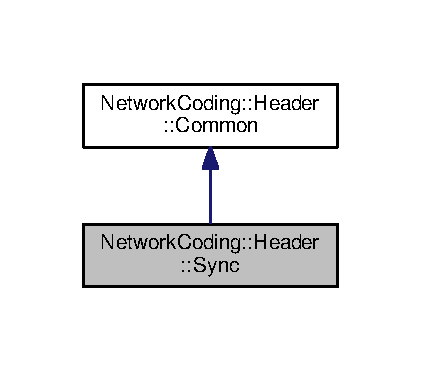
\includegraphics[width=202pt]{struct_network_coding_1_1_header_1_1_sync__inherit__graph}
\end{center}
\end{figure}


Collaboration diagram for Network\+Coding\+:\+:Header\+:\+:Sync\+:\nopagebreak
\begin{figure}[H]
\begin{center}
\leavevmode
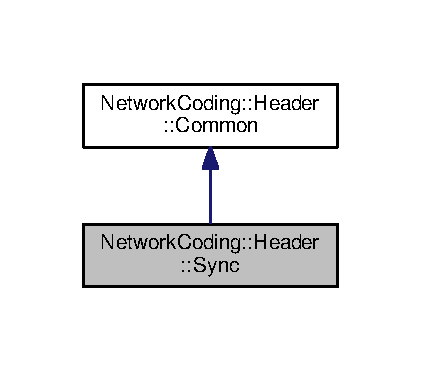
\includegraphics[width=202pt]{struct_network_coding_1_1_header_1_1_sync__coll__graph}
\end{center}
\end{figure}
\subsection*{Public Attributes}
\begin{DoxyCompactItemize}
\item 
uint16\+\_\+t {\bfseries m\+\_\+\+Sequence}\hypertarget{struct_network_coding_1_1_header_1_1_sync_a3e371d3de31efd6d519e10aa7175f6ac}{}\label{struct_network_coding_1_1_header_1_1_sync_a3e371d3de31efd6d519e10aa7175f6ac}

\end{DoxyCompactItemize}
\subsection*{Additional Inherited Members}


The documentation for this struct was generated from the following file\+:\begin{DoxyCompactItemize}
\item 
/home/dujeonglee/\+Network\+Coding\+Rev/c\+\_\+cpp/common.\+h\end{DoxyCompactItemize}

\hypertarget{class_network_coding_1_1_transmission}{}\section{Network\+Coding\+:\+:Transmission Class Reference}
\label{class_network_coding_1_1_transmission}\index{Network\+Coding\+::\+Transmission@{Network\+Coding\+::\+Transmission}}
\subsection*{Public Member Functions}
\begin{DoxyCompactItemize}
\item 
{\bfseries Transmission} (const int32\+\_\+t Socket)\hypertarget{class_network_coding_1_1_transmission_a0088c71d39d15bcbdeab5be97ca9c521}{}\label{class_network_coding_1_1_transmission_a0088c71d39d15bcbdeab5be97ca9c521}

\item 
bool {\bfseries Connect} (const \hyperlink{class_network_coding_1_1_data_types_1_1_address}{Data\+Types\+::\+Address} Addr, uint32\+\_\+t Connection\+Timeout, const Parameter\+::\+T\+R\+A\+N\+S\+M\+I\+S\+S\+I\+O\+N\+\_\+\+M\+O\+DE Transmission\+Mode, const Parameter\+::\+B\+L\+O\+C\+K\+\_\+\+S\+I\+ZE Block\+Size, const uint16\+\_\+t Retransmission\+Redundancy=0)\hypertarget{class_network_coding_1_1_transmission_acf7b8882079065561cf712db570f1a97}{}\label{class_network_coding_1_1_transmission_acf7b8882079065561cf712db570f1a97}

\item 
bool \hyperlink{class_network_coding_1_1_transmission_a374d54400d1a31f7d85119670d896aa8}{Send} (const \hyperlink{class_network_coding_1_1_data_types_1_1_address}{Data\+Types\+::\+Address} Addr, uint8\+\_\+t $\ast$const buffer, const uint16\+\_\+t buffersize)
\item 
bool {\bfseries Flush} (const \hyperlink{class_network_coding_1_1_data_types_1_1_address}{Data\+Types\+::\+Address} Addr)\hypertarget{class_network_coding_1_1_transmission_a4c843d9330d4c073e69ce82890012e6a}{}\label{class_network_coding_1_1_transmission_a4c843d9330d4c073e69ce82890012e6a}

\item 
void {\bfseries Wait\+Until\+Tx\+Is\+Completed} (const \hyperlink{class_network_coding_1_1_data_types_1_1_address}{Data\+Types\+::\+Address} Addr)\hypertarget{class_network_coding_1_1_transmission_a3b9dae872646600c26c7dd2864205d25}{}\label{class_network_coding_1_1_transmission_a3b9dae872646600c26c7dd2864205d25}

\item 
void {\bfseries Disconnect} (const \hyperlink{class_network_coding_1_1_data_types_1_1_address}{Data\+Types\+::\+Address} Addr)\hypertarget{class_network_coding_1_1_transmission_a5de9d315363eae64e7395c3d0ed6ae3b}{}\label{class_network_coding_1_1_transmission_a5de9d315363eae64e7395c3d0ed6ae3b}

\item 
void {\bfseries Rx\+Handler} (uint8\+\_\+t $\ast$const buffer, const uint16\+\_\+t size, const sockaddr $\ast$const sender\+\_\+addr, const uint32\+\_\+t sender\+\_\+addr\+\_\+len)\hypertarget{class_network_coding_1_1_transmission_ab363fc5b8d61a9fee2ab0331c1d1938e}{}\label{class_network_coding_1_1_transmission_ab363fc5b8d61a9fee2ab0331c1d1938e}

\end{DoxyCompactItemize}


\subsection{Member Function Documentation}
\index{Network\+Coding\+::\+Transmission@{Network\+Coding\+::\+Transmission}!Send@{Send}}
\index{Send@{Send}!Network\+Coding\+::\+Transmission@{Network\+Coding\+::\+Transmission}}
\subsubsection[{\texorpdfstring{Send(const Data\+Types\+::\+Address Addr, uint8\+\_\+t $\ast$const buffer, const uint16\+\_\+t buffersize)}{Send(const DataTypes::Address Addr, uint8_t *const buffer, const uint16_t buffersize)}}]{\setlength{\rightskip}{0pt plus 5cm}bool Transmission\+::\+Send (
\begin{DoxyParamCaption}
\item[{const {\bf Data\+Types\+::\+Address}}]{Addr, }
\item[{uint8\+\_\+t $\ast$const}]{buffer, }
\item[{const uint16\+\_\+t}]{buffersize}
\end{DoxyParamCaption}
)}\hypertarget{class_network_coding_1_1_transmission_a374d54400d1a31f7d85119670d896aa8}{}\label{class_network_coding_1_1_transmission_a374d54400d1a31f7d85119670d896aa8}
Block sending until there are availalbe congestion window for this packet.

The documentation for this class was generated from the following files\+:\begin{DoxyCompactItemize}
\item 
/home/dujeonglee/\+Network\+Coding\+Rev/c\+\_\+cpp/tx.\+h\item 
/home/dujeonglee/\+Network\+Coding\+Rev/c\+\_\+cpp/tx.\+cpp\end{DoxyCompactItemize}

\hypertarget{class_network_coding_1_1_transmission_block}{}\section{Network\+Coding\+:\+:Transmission\+Block Class Reference}
\label{class_network_coding_1_1_transmission_block}\index{Network\+Coding\+::\+Transmission\+Block@{Network\+Coding\+::\+Transmission\+Block}}


Network coding block.  




{\ttfamily \#include $<$tx.\+h$>$}



Collaboration diagram for Network\+Coding\+:\+:Transmission\+Block\+:\nopagebreak
\begin{figure}[H]
\begin{center}
\leavevmode
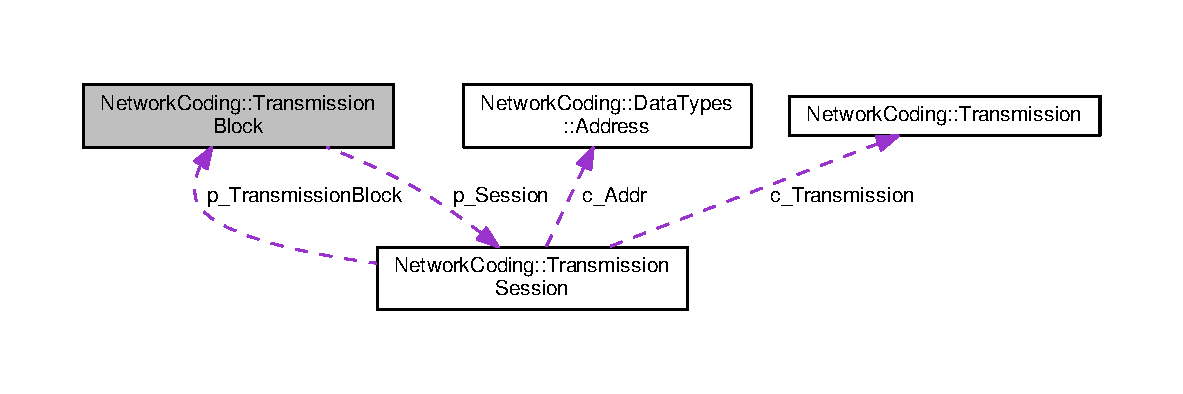
\includegraphics[width=350pt]{class_network_coding_1_1_transmission_block__coll__graph}
\end{center}
\end{figure}
\subsection*{Public Member Functions}
\begin{DoxyCompactItemize}
\item 
{\bfseries Transmission\+Block} (const \hyperlink{class_network_coding_1_1_transmission_block}{Transmission\+Block} \&)=delete\hypertarget{class_network_coding_1_1_transmission_block_a627842c53e1c3b0be511b98e85da7b02}{}\label{class_network_coding_1_1_transmission_block_a627842c53e1c3b0be511b98e85da7b02}

\item 
{\bfseries Transmission\+Block} (\hyperlink{class_network_coding_1_1_transmission_session}{Transmission\+Session} \&\&)=delete\hypertarget{class_network_coding_1_1_transmission_block_a4863f50573d5d6f2aab3c05b8f8fa6e8}{}\label{class_network_coding_1_1_transmission_block_a4863f50573d5d6f2aab3c05b8f8fa6e8}

\item 
\hyperlink{class_network_coding_1_1_transmission_block_a77977a7fed4dbf38c23a31bacc5f5e96}{Transmission\+Block} (\hyperlink{class_network_coding_1_1_transmission_session}{Transmission\+Session} $\ast$const p\+\_\+session)
\begin{DoxyCompactList}\small\item\em Construct a new \hyperlink{class_network_coding_1_1_transmission_block}{Transmission\+Block} object. \end{DoxyCompactList}\item 
\hyperlink{class_network_coding_1_1_transmission_block_a7a001dfa2611c27d3cedbcdcd292c927}{$\sim$\+Transmission\+Block} ()
\begin{DoxyCompactList}\small\item\em Destroy the \hyperlink{class_network_coding_1_1_transmission}{Transmission} Block object. \end{DoxyCompactList}\item 
\hyperlink{class_network_coding_1_1_transmission_block}{Transmission\+Block} \& {\bfseries operator=} (const \hyperlink{class_network_coding_1_1_transmission_block}{Transmission\+Block} \&)=delete\hypertarget{class_network_coding_1_1_transmission_block_adece22af088c127c18822d42d0f0e053}{}\label{class_network_coding_1_1_transmission_block_adece22af088c127c18822d42d0f0e053}

\item 
\hyperlink{class_network_coding_1_1_transmission_block}{Transmission\+Block} \& {\bfseries operator=} (\hyperlink{class_network_coding_1_1_transmission_block}{Transmission\+Block} \&\&)=delete\hypertarget{class_network_coding_1_1_transmission_block_af0cc440e659421ce4d0c4b90a293a8fd}{}\label{class_network_coding_1_1_transmission_block_af0cc440e659421ce4d0c4b90a293a8fd}

\item 
bool \hyperlink{class_network_coding_1_1_transmission_block_a4a372836698727d1cd31e0e353198318}{Send} (uint8\+\_\+t $\ast$const buffer, const uint16\+\_\+t buffersize)
\begin{DoxyCompactList}\small\item\em Enqueue a packet into a transmission buffer of the relavent session. \end{DoxyCompactList}\item 
const bool \hyperlink{class_network_coding_1_1_transmission_block_ad8d4de3ed6b6dda67a09afb1c7760ac3}{Retransmission} ()
\begin{DoxyCompactList}\small\item\em Transmit a remedy packet. \end{DoxyCompactList}\end{DoxyCompactItemize}
\subsection*{Public Attributes}
\begin{DoxyCompactItemize}
\item 
\hyperlink{class_network_coding_1_1_transmission_session}{Transmission\+Session} $\ast$const \hyperlink{class_network_coding_1_1_transmission_block_ae45d8369907e22b369bc8d0a0d93d378}{p\+\_\+\+Session}\hypertarget{class_network_coding_1_1_transmission_block_ae45d8369907e22b369bc8d0a0d93d378}{}\label{class_network_coding_1_1_transmission_block_ae45d8369907e22b369bc8d0a0d93d378}

\begin{DoxyCompactList}\small\item\em Pointer of the \hyperlink{class_network_coding_1_1_transmission_session}{Transmission\+Session} object that this block is associated. \end{DoxyCompactList}\item 
const uint8\+\_\+t \hyperlink{class_network_coding_1_1_transmission_block_a3fac24ea69bc7f68f297d72f0b3e0448}{m\+\_\+\+Block\+Size}
\begin{DoxyCompactList}\small\item\em Block size. \end{DoxyCompactList}\item 
const uint8\+\_\+t \hyperlink{class_network_coding_1_1_transmission_block_a82c18d348f0a5660240e47ee9c9880b1}{m\+\_\+\+Transmission\+Mode}
\begin{DoxyCompactList}\small\item\em Mode. \end{DoxyCompactList}\item 
const uint16\+\_\+t \hyperlink{class_network_coding_1_1_transmission_block_a54d1c096df401da6ca57636c91b3faca}{m\+\_\+\+Block\+Sequence\+Number}
\begin{DoxyCompactList}\small\item\em The sequence number of this block. Each block has unique sequence number. The sequence number is incremented by one in the next block. \end{DoxyCompactList}\item 
const uint16\+\_\+t \hyperlink{class_network_coding_1_1_transmission_block_a1dc8966af67de1e8309b62e3f87854f2}{m\+\_\+\+Retransmission\+Redundancy}
\begin{DoxyCompactList}\small\item\em Maximum number of remedy packets. It is valid only when mode is B\+E\+S\+T\+\_\+\+E\+F\+F\+O\+R\+T\+\_\+\+T\+R\+A\+N\+S\+M\+I\+S\+S\+I\+O\+N\+\_\+\+M\+O\+DE. \end{DoxyCompactList}\item 
uint16\+\_\+t \hyperlink{class_network_coding_1_1_transmission_block_adcc79e6bfd7282430f95268ec86369a7}{m\+\_\+\+Largest\+Original\+Packet\+Size}
\begin{DoxyCompactList}\small\item\em The largest packet size in this block, i.\+e., encoding packet size. \end{DoxyCompactList}\item 
uint8\+\_\+t \hyperlink{class_network_coding_1_1_transmission_block_a84e8b076ce5fea10351626094003cd33}{m\+\_\+\+Transmission\+Count}\hypertarget{class_network_coding_1_1_transmission_block_a84e8b076ce5fea10351626094003cd33}{}\label{class_network_coding_1_1_transmission_block_a84e8b076ce5fea10351626094003cd33}

\begin{DoxyCompactList}\small\item\em The nunber of transmission including retranmission. \end{DoxyCompactList}\item 
uint8\+\_\+t \hyperlink{class_network_coding_1_1_transmission_block_a9277a19ef3f5e5d9ecf2b7e91ee1c1dd}{m\+\_\+\+Acked\+Rank}\hypertarget{class_network_coding_1_1_transmission_block_a9277a19ef3f5e5d9ecf2b7e91ee1c1dd}{}\label{class_network_coding_1_1_transmission_block_a9277a19ef3f5e5d9ecf2b7e91ee1c1dd}

\begin{DoxyCompactList}\small\item\em Acknowleged rank from receiver. m\+\_\+\+Acked\+Rank == m\+\_\+\+Block\+Size means that receiver has recovered all of the packets in this block. \end{DoxyCompactList}\item 
uint8\+\_\+t \hyperlink{class_network_coding_1_1_transmission_block_a15538df05b3b58218d43363e8b59f27c}{m\+\_\+\+Remedy\+Packet\+Buffer} \mbox{[}Parameter\+::\+M\+A\+X\+I\+M\+U\+M\+\_\+\+B\+U\+F\+F\+E\+R\+\_\+\+S\+I\+ZE\mbox{]}\hypertarget{class_network_coding_1_1_transmission_block_a15538df05b3b58218d43363e8b59f27c}{}\label{class_network_coding_1_1_transmission_block_a15538df05b3b58218d43363e8b59f27c}

\begin{DoxyCompactList}\small\item\em Remedy packet buffer. \end{DoxyCompactList}\item 
std\+::vector$<$ std\+::unique\+\_\+ptr$<$ uint8\+\_\+t\mbox{[}$\,$\mbox{]}$>$ $>$ \hyperlink{class_network_coding_1_1_transmission_block_aeefe661df0123d02bb1fc463136d2fe5}{m\+\_\+\+Original\+Packet\+Buffer}\hypertarget{class_network_coding_1_1_transmission_block_aeefe661df0123d02bb1fc463136d2fe5}{}\label{class_network_coding_1_1_transmission_block_aeefe661df0123d02bb1fc463136d2fe5}

\begin{DoxyCompactList}\small\item\em An array of original packets. The size of array should be match with m\+\_\+\+Block\+Size. \end{DoxyCompactList}\end{DoxyCompactItemize}


\subsection{Detailed Description}
Network coding block. 

\subsection{Constructor \& Destructor Documentation}
\index{Network\+Coding\+::\+Transmission\+Block@{Network\+Coding\+::\+Transmission\+Block}!Transmission\+Block@{Transmission\+Block}}
\index{Transmission\+Block@{Transmission\+Block}!Network\+Coding\+::\+Transmission\+Block@{Network\+Coding\+::\+Transmission\+Block}}
\subsubsection[{\texorpdfstring{Transmission\+Block(\+Transmission\+Session $\ast$const p\+\_\+session)}{TransmissionBlock(TransmissionSession *const p_session)}}]{\setlength{\rightskip}{0pt plus 5cm}Transmission\+Block\+::\+Transmission\+Block (
\begin{DoxyParamCaption}
\item[{{\bf Transmission\+Session} $\ast$const}]{p\+\_\+session}
\end{DoxyParamCaption}
)}\hypertarget{class_network_coding_1_1_transmission_block_a77977a7fed4dbf38c23a31bacc5f5e96}{}\label{class_network_coding_1_1_transmission_block_a77977a7fed4dbf38c23a31bacc5f5e96}


Construct a new \hyperlink{class_network_coding_1_1_transmission_block}{Transmission\+Block} object. 


\begin{DoxyParams}{Parameters}
{\em p\+\_\+session} & \+: Pointer of the \hyperlink{class_network_coding_1_1_transmission_session}{Transmission\+Session} object that this block is associated. \\
\hline
\end{DoxyParams}

\begin{DoxyEnumerate}
\item Initialize the member variables.
\item Register the block sequence number to \hyperlink{class_network_coding_1_1_transmission_session_aa7b466f696587e66d2a961701d552a6a}{Network\+Coding\+::\+Transmission\+Session\+::m\+\_\+\+Ack\+List}. \begin{DoxySeeAlso}{See also}
\hyperlink{class_network_coding_1_1_transmission_session_aa7b466f696587e66d2a961701d552a6a}{Network\+Coding\+::\+Transmission\+Session\+::m\+\_\+\+Ack\+List}.
\end{DoxySeeAlso}

\end{DoxyEnumerate}\index{Network\+Coding\+::\+Transmission\+Block@{Network\+Coding\+::\+Transmission\+Block}!````~Transmission\+Block@{$\sim$\+Transmission\+Block}}
\index{````~Transmission\+Block@{$\sim$\+Transmission\+Block}!Network\+Coding\+::\+Transmission\+Block@{Network\+Coding\+::\+Transmission\+Block}}
\subsubsection[{\texorpdfstring{$\sim$\+Transmission\+Block()}{~TransmissionBlock()}}]{\setlength{\rightskip}{0pt plus 5cm}Transmission\+Block\+::$\sim$\+Transmission\+Block (
\begin{DoxyParamCaption}
{}
\end{DoxyParamCaption}
)}\hypertarget{class_network_coding_1_1_transmission_block_a7a001dfa2611c27d3cedbcdcd292c927}{}\label{class_network_coding_1_1_transmission_block_a7a001dfa2611c27d3cedbcdcd292c927}


Destroy the \hyperlink{class_network_coding_1_1_transmission}{Transmission} Block object. 


\begin{DoxyEnumerate}
\item Update \hyperlink{class_network_coding_1_1_transmission_session_a27ee5813374da47482b72295b85548f4}{Network\+Coding\+::\+Transmission\+Session\+::m\+\_\+\+Bytes\+Unacked}. \begin{DoxySeeAlso}{See also}
\hyperlink{class_network_coding_1_1_transmission_session_a27ee5813374da47482b72295b85548f4}{Network\+Coding\+::\+Transmission\+Session\+::m\+\_\+\+Bytes\+Unacked}.
\end{DoxySeeAlso}

\item Clear \hyperlink{class_network_coding_1_1_transmission_block_aeefe661df0123d02bb1fc463136d2fe5}{Network\+Coding\+::\+Transmission\+Block\+::m\+\_\+\+Original\+Packet\+Buffer}. \begin{DoxySeeAlso}{See also}
\hyperlink{class_network_coding_1_1_transmission_block_aeefe661df0123d02bb1fc463136d2fe5}{Network\+Coding\+::\+Transmission\+Block\+::m\+\_\+\+Original\+Packet\+Buffer}.
\end{DoxySeeAlso}

\end{DoxyEnumerate}

\subsection{Member Function Documentation}
\index{Network\+Coding\+::\+Transmission\+Block@{Network\+Coding\+::\+Transmission\+Block}!Retransmission@{Retransmission}}
\index{Retransmission@{Retransmission}!Network\+Coding\+::\+Transmission\+Block@{Network\+Coding\+::\+Transmission\+Block}}
\subsubsection[{\texorpdfstring{Retransmission()}{Retransmission()}}]{\setlength{\rightskip}{0pt plus 5cm}const bool Transmission\+Block\+::\+Retransmission (
\begin{DoxyParamCaption}
{}
\end{DoxyParamCaption}
)}\hypertarget{class_network_coding_1_1_transmission_block_ad8d4de3ed6b6dda67a09afb1c7760ac3}{}\label{class_network_coding_1_1_transmission_block_ad8d4de3ed6b6dda67a09afb1c7760ac3}


Transmit a remedy packet. 

\begin{DoxyReturn}{Returns}
true \+: Remedy packet has been successfully transmitted. 

false \+: Either receiver has received all of the packets for this block or connection is lost. 
\end{DoxyReturn}

\begin{DoxyEnumerate}
\item If \hyperlink{class_network_coding_1_1_transmission_block_a82c18d348f0a5660240e47ee9c9880b1}{Network\+Coding\+::\+Transmission\+Block\+::m\+\_\+\+Transmission\+Mode} is Network\+Coding\+::\+Parameter\+::\+B\+E\+S\+T\+\_\+\+E\+F\+F\+O\+R\+T\+\_\+\+T\+R\+A\+N\+S\+M\+I\+S\+S\+I\+O\+N\+\_\+\+M\+O\+DE and we already transmitted \hyperlink{class_network_coding_1_1_transmission_block_a1dc8966af67de1e8309b62e3f87854f2}{Network\+Coding\+::\+Transmission\+Block\+::m\+\_\+\+Retransmission\+Redundancy} remedy packets then we complete this block regardless of ack from receiver.
\item Update \hyperlink{class_network_coding_1_1_transmission_session_a3c5449f03555c74ccff2e4d0b99c13d9}{Network\+Coding\+::\+Transmission\+Session\+::m\+\_\+\+Min\+Block\+Sequence\+Number} with the minimum sequence number in \hyperlink{class_network_coding_1_1_transmission_session_aa7b466f696587e66d2a961701d552a6a}{Network\+Coding\+::\+Transmission\+Session\+::m\+\_\+\+Ack\+List}. \begin{DoxyWarning}{Warning}
$\sim$\+Transmission\+Block require m\+\_\+\+Ack\+List\+Lock. Therefore, we must release m\+\_\+\+Ack\+List\+Lock before calling dtor.
\end{DoxyWarning}

\item Check if session is in connected state.
\item Generate random coefficients. If m\+\_\+\+Original\+Packet\+Buffer.\+size() == 1 we do not encode the packet. Otherwise, we generates m\+\_\+\+Original\+Packet\+Buffer.\+size() many random coefficients.
\item Prepare header. \begin{DoxySeeAlso}{See also}
\hyperlink{struct_network_coding_1_1_header_1_1_data}{Network\+Coding\+::\+Header\+::\+Data}.
\end{DoxySeeAlso}

\item Encoding a remedy packet.
\item Enqueue the remedy packet. \begin{DoxySeeAlso}{See also}
\hyperlink{class_network_coding_1_1_transmission_session_ae248b2c48a54243ce1e47837337231df}{Network\+Coding\+::\+Transmission\+Session\+::\+Push\+Data\+Packet}.
\end{DoxySeeAlso}

\end{DoxyEnumerate}\index{Network\+Coding\+::\+Transmission\+Block@{Network\+Coding\+::\+Transmission\+Block}!Send@{Send}}
\index{Send@{Send}!Network\+Coding\+::\+Transmission\+Block@{Network\+Coding\+::\+Transmission\+Block}}
\subsubsection[{\texorpdfstring{Send(uint8\+\_\+t $\ast$const buffer, const uint16\+\_\+t buffersize)}{Send(uint8_t *const buffer, const uint16_t buffersize)}}]{\setlength{\rightskip}{0pt plus 5cm}bool Transmission\+Block\+::\+Send (
\begin{DoxyParamCaption}
\item[{uint8\+\_\+t $\ast$const}]{buffer, }
\item[{const uint16\+\_\+t}]{buffersize}
\end{DoxyParamCaption}
)}\hypertarget{class_network_coding_1_1_transmission_block_a4a372836698727d1cd31e0e353198318}{}\label{class_network_coding_1_1_transmission_block_a4a372836698727d1cd31e0e353198318}


Enqueue a packet into a transmission buffer of the relavent session. 

\begin{DoxySeeAlso}{See also}
\hyperlink{class_network_coding_1_1_transmission_session_ae248b2c48a54243ce1e47837337231df}{Network\+Coding\+::\+Transmission\+Session\+::\+Push\+Data\+Packet} 
\end{DoxySeeAlso}

\begin{DoxyParams}{Parameters}
{\em buffer} & \+: Buffer for transmission. \\
\hline
{\em buffersize} & \+: Size of the buffer. \\
\hline
\end{DoxyParams}
\begin{DoxyReturn}{Returns}
true \+: Success 

false \+: Failure 
\end{DoxyReturn}

\begin{DoxyEnumerate}
\item Check if session is in connected state. \begin{DoxySeeAlso}{See also}
\hyperlink{class_network_coding_1_1_transmission_session_aa12eab14f68b6e4dc5e2de25ff017282}{Network\+Coding\+::\+Transmission\+Session\+::m\+\_\+\+Is\+Connected}.
\end{DoxySeeAlso}

\item Put buffer into the m\+\_\+\+Original\+Packet\+Buffer. \begin{DoxySeeAlso}{See also}
\hyperlink{class_network_coding_1_1_transmission_block_aeefe661df0123d02bb1fc463136d2fe5}{Network\+Coding\+::\+Transmission\+Block\+::m\+\_\+\+Original\+Packet\+Buffer}.
\end{DoxySeeAlso}

\item Prepare header. \begin{DoxySeeAlso}{See also}
\hyperlink{struct_network_coding_1_1_header_1_1_data}{Network\+Coding\+::\+Header\+::\+Data}.
\end{DoxySeeAlso}

\item Enqueue the packet. \begin{DoxySeeAlso}{See also}
\hyperlink{class_network_coding_1_1_transmission_session_ae248b2c48a54243ce1e47837337231df}{Network\+Coding\+::\+Transmission\+Session\+::\+Push\+Data\+Packet}.
\end{DoxySeeAlso}

\item Clear \hyperlink{class_network_coding_1_1_transmission_session_acc18d6b10a856b3dfda76c7b85899911}{Network\+Coding\+::\+Transmission\+Session\+::p\+\_\+\+Transmission\+Block} so that \hyperlink{class_network_coding_1_1_transmission_session}{Network\+Coding\+::\+Transmission\+Session} can arrange next block for transmission. \begin{DoxySeeAlso}{See also}
\hyperlink{class_network_coding_1_1_transmission_session_acc18d6b10a856b3dfda76c7b85899911}{Network\+Coding\+::\+Transmission\+Session\+::p\+\_\+\+Transmission\+Block}.
\end{DoxySeeAlso}

\end{DoxyEnumerate}

\subsection{Member Data Documentation}
\index{Network\+Coding\+::\+Transmission\+Block@{Network\+Coding\+::\+Transmission\+Block}!m\+\_\+\+Block\+Sequence\+Number@{m\+\_\+\+Block\+Sequence\+Number}}
\index{m\+\_\+\+Block\+Sequence\+Number@{m\+\_\+\+Block\+Sequence\+Number}!Network\+Coding\+::\+Transmission\+Block@{Network\+Coding\+::\+Transmission\+Block}}
\subsubsection[{\texorpdfstring{m\+\_\+\+Block\+Sequence\+Number}{m_BlockSequenceNumber}}]{\setlength{\rightskip}{0pt plus 5cm}const uint16\+\_\+t Network\+Coding\+::\+Transmission\+Block\+::m\+\_\+\+Block\+Sequence\+Number}\hypertarget{class_network_coding_1_1_transmission_block_a54d1c096df401da6ca57636c91b3faca}{}\label{class_network_coding_1_1_transmission_block_a54d1c096df401da6ca57636c91b3faca}


The sequence number of this block. Each block has unique sequence number. The sequence number is incremented by one in the next block. 

\begin{DoxyWarning}{Warning}
This member should be constant value. 
\end{DoxyWarning}
\index{Network\+Coding\+::\+Transmission\+Block@{Network\+Coding\+::\+Transmission\+Block}!m\+\_\+\+Block\+Size@{m\+\_\+\+Block\+Size}}
\index{m\+\_\+\+Block\+Size@{m\+\_\+\+Block\+Size}!Network\+Coding\+::\+Transmission\+Block@{Network\+Coding\+::\+Transmission\+Block}}
\subsubsection[{\texorpdfstring{m\+\_\+\+Block\+Size}{m_BlockSize}}]{\setlength{\rightskip}{0pt plus 5cm}const uint8\+\_\+t Network\+Coding\+::\+Transmission\+Block\+::m\+\_\+\+Block\+Size}\hypertarget{class_network_coding_1_1_transmission_block_a3fac24ea69bc7f68f297d72f0b3e0448}{}\label{class_network_coding_1_1_transmission_block_a3fac24ea69bc7f68f297d72f0b3e0448}


Block size. 

\begin{DoxySeeAlso}{See also}
Network\+Coding\+::\+Parameter\+::\+B\+L\+O\+C\+K\+\_\+\+S\+I\+ZE. 
\end{DoxySeeAlso}
\begin{DoxyWarning}{Warning}
This member should be constant value. 
\end{DoxyWarning}
\index{Network\+Coding\+::\+Transmission\+Block@{Network\+Coding\+::\+Transmission\+Block}!m\+\_\+\+Largest\+Original\+Packet\+Size@{m\+\_\+\+Largest\+Original\+Packet\+Size}}
\index{m\+\_\+\+Largest\+Original\+Packet\+Size@{m\+\_\+\+Largest\+Original\+Packet\+Size}!Network\+Coding\+::\+Transmission\+Block@{Network\+Coding\+::\+Transmission\+Block}}
\subsubsection[{\texorpdfstring{m\+\_\+\+Largest\+Original\+Packet\+Size}{m_LargestOriginalPacketSize}}]{\setlength{\rightskip}{0pt plus 5cm}uint16\+\_\+t Network\+Coding\+::\+Transmission\+Block\+::m\+\_\+\+Largest\+Original\+Packet\+Size}\hypertarget{class_network_coding_1_1_transmission_block_adcc79e6bfd7282430f95268ec86369a7}{}\label{class_network_coding_1_1_transmission_block_adcc79e6bfd7282430f95268ec86369a7}


The largest packet size in this block, i.\+e., encoding packet size. 

\begin{DoxyWarning}{Warning}
m\+\_\+\+Largest\+Original\+Packet\+Size should be less than M\+A\+X\+I\+M\+U\+M\+\_\+\+B\+U\+F\+F\+E\+R\+\_\+\+S\+I\+ZE. 
\end{DoxyWarning}
\index{Network\+Coding\+::\+Transmission\+Block@{Network\+Coding\+::\+Transmission\+Block}!m\+\_\+\+Retransmission\+Redundancy@{m\+\_\+\+Retransmission\+Redundancy}}
\index{m\+\_\+\+Retransmission\+Redundancy@{m\+\_\+\+Retransmission\+Redundancy}!Network\+Coding\+::\+Transmission\+Block@{Network\+Coding\+::\+Transmission\+Block}}
\subsubsection[{\texorpdfstring{m\+\_\+\+Retransmission\+Redundancy}{m_RetransmissionRedundancy}}]{\setlength{\rightskip}{0pt plus 5cm}const uint16\+\_\+t Network\+Coding\+::\+Transmission\+Block\+::m\+\_\+\+Retransmission\+Redundancy}\hypertarget{class_network_coding_1_1_transmission_block_a1dc8966af67de1e8309b62e3f87854f2}{}\label{class_network_coding_1_1_transmission_block_a1dc8966af67de1e8309b62e3f87854f2}


Maximum number of remedy packets. It is valid only when mode is B\+E\+S\+T\+\_\+\+E\+F\+F\+O\+R\+T\+\_\+\+T\+R\+A\+N\+S\+M\+I\+S\+S\+I\+O\+N\+\_\+\+M\+O\+DE. 

\begin{DoxySeeAlso}{See also}
Network\+Coding\+::\+Parameter\+::\+T\+R\+A\+N\+S\+M\+I\+S\+S\+I\+O\+N\+\_\+\+M\+O\+DE. 
\end{DoxySeeAlso}
\begin{DoxyWarning}{Warning}
This member should be constant value. 
\end{DoxyWarning}
\index{Network\+Coding\+::\+Transmission\+Block@{Network\+Coding\+::\+Transmission\+Block}!m\+\_\+\+Transmission\+Mode@{m\+\_\+\+Transmission\+Mode}}
\index{m\+\_\+\+Transmission\+Mode@{m\+\_\+\+Transmission\+Mode}!Network\+Coding\+::\+Transmission\+Block@{Network\+Coding\+::\+Transmission\+Block}}
\subsubsection[{\texorpdfstring{m\+\_\+\+Transmission\+Mode}{m_TransmissionMode}}]{\setlength{\rightskip}{0pt plus 5cm}const uint8\+\_\+t Network\+Coding\+::\+Transmission\+Block\+::m\+\_\+\+Transmission\+Mode}\hypertarget{class_network_coding_1_1_transmission_block_a82c18d348f0a5660240e47ee9c9880b1}{}\label{class_network_coding_1_1_transmission_block_a82c18d348f0a5660240e47ee9c9880b1}


Mode. 

\begin{DoxySeeAlso}{See also}
Network\+Coding\+::\+Parameter\+::\+T\+R\+A\+N\+S\+M\+I\+S\+S\+I\+O\+N\+\_\+\+M\+O\+DE. 
\end{DoxySeeAlso}
\begin{DoxyWarning}{Warning}
This member should be constant value. 
\end{DoxyWarning}


The documentation for this class was generated from the following files\+:\begin{DoxyCompactItemize}
\item 
/home/dujeonglee/\+Network\+Coding\+Rev/c\+\_\+cpp/tx.\+h\item 
/home/dujeonglee/\+Network\+Coding\+Rev/c\+\_\+cpp/tx.\+cpp\end{DoxyCompactItemize}

\hypertarget{class_network_coding_1_1_transmission_session}{}\section{Network\+Coding\+:\+:Transmission\+Session Class Reference}
\label{class_network_coding_1_1_transmission_session}\index{Network\+Coding\+::\+Transmission\+Session@{Network\+Coding\+::\+Transmission\+Session}}


Network coding session.  




{\ttfamily \#include $<$tx.\+h$>$}



Collaboration diagram for Network\+Coding\+:\+:Transmission\+Session\+:\nopagebreak
\begin{figure}[H]
\begin{center}
\leavevmode
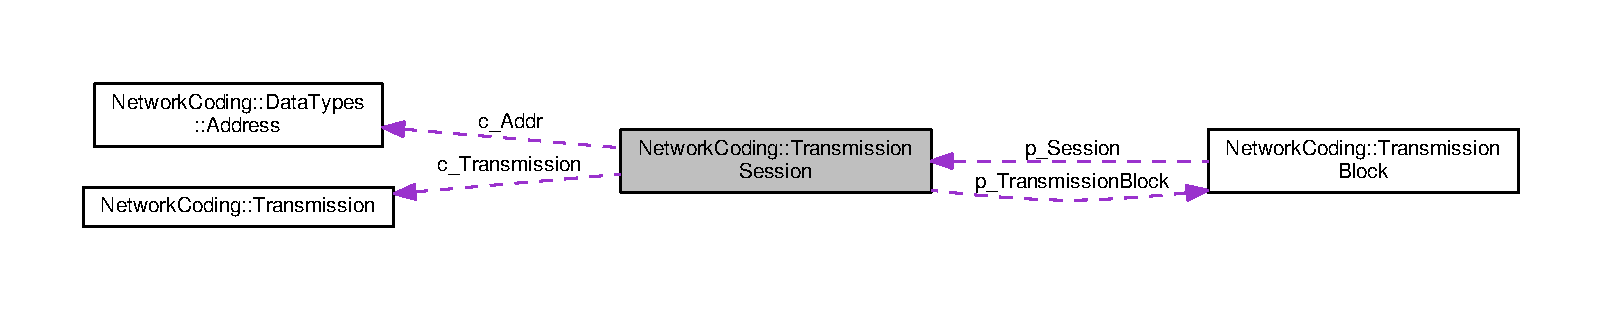
\includegraphics[width=350pt]{class_network_coding_1_1_transmission_session__coll__graph}
\end{center}
\end{figure}
\subsection*{Public Types}
\begin{DoxyCompactItemize}
\item 
enum \hyperlink{class_network_coding_1_1_transmission_session_aa224de09cc46cfd07df11e4ddeff7472}{Task\+Priority} \{ {\bfseries H\+I\+G\+H\+\_\+\+P\+R\+I\+O\+R\+I\+TY} = 0, 
{\bfseries M\+I\+D\+D\+L\+E\+\_\+\+P\+R\+I\+O\+R\+I\+TY}, 
{\bfseries L\+O\+W\+\_\+\+P\+R\+I\+O\+R\+I\+TY}, 
{\bfseries P\+R\+I\+O\+R\+I\+T\+Y\+\_\+\+L\+E\+V\+E\+LS}
 \}\hypertarget{class_network_coding_1_1_transmission_session_aa224de09cc46cfd07df11e4ddeff7472}{}\label{class_network_coding_1_1_transmission_session_aa224de09cc46cfd07df11e4ddeff7472}
\begin{DoxyCompactList}\small\item\em $<$ Priority of lambda task queued on m\+\_\+\+Timer. \end{DoxyCompactList}
\end{DoxyCompactItemize}
\subsection*{Public Member Functions}
\begin{DoxyCompactItemize}
\item 
\hyperlink{class_network_coding_1_1_transmission_session_a4ab773a704ec3740cbf222cad7e45262}{Transmission\+Session} (\hyperlink{class_network_coding_1_1_transmission}{Transmission} $\ast$const transmission, const int32\+\_\+t Socket, const \hyperlink{class_network_coding_1_1_data_types_1_1_address}{Data\+Types\+::\+Address} Addr, const Parameter\+::\+T\+R\+A\+N\+S\+M\+I\+S\+S\+I\+O\+N\+\_\+\+M\+O\+DE Transmission\+Mode=Parameter\+::\+T\+R\+A\+N\+S\+M\+I\+S\+S\+I\+O\+N\+\_\+\+M\+O\+D\+E\+::\+R\+E\+L\+I\+A\+B\+L\+E\+\_\+\+T\+R\+A\+N\+S\+M\+I\+S\+S\+I\+O\+N\+\_\+\+M\+O\+DE, const Parameter\+::\+B\+L\+O\+C\+K\+\_\+\+S\+I\+ZE Block\+Size=Parameter\+::\+B\+L\+O\+C\+K\+\_\+\+S\+I\+Z\+E\+::\+B\+L\+O\+C\+K\+\_\+\+S\+I\+Z\+E\+\_\+04, const uint16\+\_\+t Retransmission\+Redundancy=0)
\begin{DoxyCompactList}\small\item\em Construct a new \hyperlink{class_network_coding_1_1_transmission_session}{Transmission\+Session} object. \end{DoxyCompactList}\item 
{\bfseries Transmission\+Session} (const \hyperlink{class_network_coding_1_1_transmission_session}{Transmission\+Session} \&)=delete\hypertarget{class_network_coding_1_1_transmission_session_ad6ea42437c5b6233d5785fe6c2126c1b}{}\label{class_network_coding_1_1_transmission_session_ad6ea42437c5b6233d5785fe6c2126c1b}

\item 
{\bfseries Transmission\+Session} (\hyperlink{class_network_coding_1_1_transmission_session}{Transmission\+Session} \&\&)=delete\hypertarget{class_network_coding_1_1_transmission_session_a455fee7d9cb4c90bacb304ad37373548}{}\label{class_network_coding_1_1_transmission_session_a455fee7d9cb4c90bacb304ad37373548}

\item 
\hyperlink{class_network_coding_1_1_transmission_session_a56c1ac128002a5e5e554511dba2d6a1d}{$\sim$\+Transmission\+Session} ()
\begin{DoxyCompactList}\small\item\em Destroy the \hyperlink{class_network_coding_1_1_transmission_session}{Transmission\+Session} object. \end{DoxyCompactList}\item 
\hyperlink{class_network_coding_1_1_transmission_session}{Transmission\+Session} \& {\bfseries operator=} (const \hyperlink{class_network_coding_1_1_transmission_session}{Transmission\+Session} \&)=delete\hypertarget{class_network_coding_1_1_transmission_session_a9005d3d1bfb5e5ef8b0a3c01f1426406}{}\label{class_network_coding_1_1_transmission_session_a9005d3d1bfb5e5ef8b0a3c01f1426406}

\item 
\hyperlink{class_network_coding_1_1_transmission_session}{Transmission\+Session} \& {\bfseries operator=} (\hyperlink{class_network_coding_1_1_transmission_session}{Transmission\+Session} \&\&)=delete\hypertarget{class_network_coding_1_1_transmission_session_a51b0867e33647c0f0556992d4a099829}{}\label{class_network_coding_1_1_transmission_session_a51b0867e33647c0f0556992d4a099829}

\item 
void \hyperlink{class_network_coding_1_1_transmission_session_a99838e572cbc7b5876d59d767e399a4e}{Change\+Transmission\+Mode} (const Parameter\+::\+T\+R\+A\+N\+S\+M\+I\+S\+S\+I\+O\+N\+\_\+\+M\+O\+DE Transmission\+Mode)
\begin{DoxyCompactList}\small\item\em Change transmission mode. The change will take effect from the next \hyperlink{class_network_coding_1_1_transmission_block}{Transmission\+Block}. \end{DoxyCompactList}\item 
void \hyperlink{class_network_coding_1_1_transmission_session_aaeb60cbe08b7ba62291dbfff17ed987d}{Change\+Block\+Size} (const Parameter\+::\+B\+L\+O\+C\+K\+\_\+\+S\+I\+ZE Block\+Size)
\begin{DoxyCompactList}\small\item\em Change block size. The change will take effect from the next \hyperlink{class_network_coding_1_1_transmission_block}{Transmission\+Block}. \end{DoxyCompactList}\item 
void \hyperlink{class_network_coding_1_1_transmission_session_ae3d21866fedfd756de3d7ab6d2151ec4}{Change\+Retransmission\+Redundancy} (const uint16\+\_\+t Retransmission\+Redundancy)
\begin{DoxyCompactList}\small\item\em Change retransmission redundancy. Retransmission redundancy is only valid for B\+E\+S\+T\+\_\+\+E\+F\+F\+O\+R\+T\+\_\+\+T\+R\+A\+N\+S\+M\+I\+S\+S\+I\+O\+N\+\_\+\+M\+O\+DE. The change will take effect from the next \hyperlink{class_network_coding_1_1_transmission_block}{Transmission\+Block}. \end{DoxyCompactList}\item 
void \hyperlink{class_network_coding_1_1_transmission_session_a4a2f5696da8bd656d1b250d2319f1212}{Change\+Session\+Parameter} (const Parameter\+::\+T\+R\+A\+N\+S\+M\+I\+S\+S\+I\+O\+N\+\_\+\+M\+O\+DE Transmission\+Mode, const Parameter\+::\+B\+L\+O\+C\+K\+\_\+\+S\+I\+ZE Block\+Size, const uint16\+\_\+t Retransmission\+Redundancy)
\begin{DoxyCompactList}\small\item\em Change the above session parameters at the same time. The changes will take effect from the next \hyperlink{class_network_coding_1_1_transmission_block}{Transmission\+Block}. \end{DoxyCompactList}\item 
const bool \hyperlink{class_network_coding_1_1_transmission_session_a732d177580449a1473cea103465b1c5b}{Send\+Ping} ()
\begin{DoxyCompactList}\small\item\em Send ping packet to the remote host. \end{DoxyCompactList}\item 
void \hyperlink{class_network_coding_1_1_transmission_session_a208883657ae7c03b6405fd949bc06d7a}{Process\+Pong} (const uint16\+\_\+t Rtt)
\begin{DoxyCompactList}\small\item\em Process pong packet. \end{DoxyCompactList}\item 
void \hyperlink{class_network_coding_1_1_transmission_session_a31f038cb688e2e95e40f63821baf34a8}{Process\+Data\+Ack} (const uint8\+\_\+t Rank, const uint8\+\_\+t Max\+Rank, const uint8\+\_\+t Loss, const uint16\+\_\+t Sequence)
\begin{DoxyCompactList}\small\item\em Process ack. \end{DoxyCompactList}\item 
void \hyperlink{class_network_coding_1_1_transmission_session_adf9cb35f78ec3f03d92ec4d46faa1c66}{Process\+Sync\+Ack} (const uint16\+\_\+t sequence)
\begin{DoxyCompactList}\small\item\em Process ack sync. \end{DoxyCompactList}\item 
void \hyperlink{class_network_coding_1_1_transmission_session_ae248b2c48a54243ce1e47837337231df}{Push\+Data\+Packet} (uint8\+\_\+t $\ast$const buffer, const uint16\+\_\+t size, bool orig, \hyperlink{class_network_coding_1_1_transmission_block}{Transmission\+Block} $\ast$const block)
\begin{DoxyCompactList}\small\item\em Enqueue a packet into m\+\_\+\+Tx\+Queue for transmission. \end{DoxyCompactList}\item 
uint16\+\_\+t \hyperlink{class_network_coding_1_1_transmission_session_adeda0f8096e8fa5845d4f0377193cf73}{Pop\+Data\+Packet} ()
\begin{DoxyCompactList}\small\item\em Dequeue a packet from m\+\_\+\+Tx\+Queue and transmit the packet. \end{DoxyCompactList}\end{DoxyCompactItemize}
\subsection*{Public Attributes}
\begin{DoxyCompactItemize}
\item 
\hyperlink{class_network_coding_1_1_transmission}{Transmission} $\ast$const \hyperlink{class_network_coding_1_1_transmission_session_a76808b9fb4d31f1c471ef313e50aff54}{c\+\_\+\+Transmission}\hypertarget{class_network_coding_1_1_transmission_session_a76808b9fb4d31f1c471ef313e50aff54}{}\label{class_network_coding_1_1_transmission_session_a76808b9fb4d31f1c471ef313e50aff54}

\begin{DoxyCompactList}\small\item\em Pointer of the \hyperlink{class_network_coding_1_1_transmission}{Transmission} object that this session is associated. \end{DoxyCompactList}\item 
const int32\+\_\+t \hyperlink{class_network_coding_1_1_transmission_session_a9d0373f0889c3f9ed0cead43c8cfefa9}{c\+\_\+\+Socket}\hypertarget{class_network_coding_1_1_transmission_session_a9d0373f0889c3f9ed0cead43c8cfefa9}{}\label{class_network_coding_1_1_transmission_session_a9d0373f0889c3f9ed0cead43c8cfefa9}

\begin{DoxyCompactList}\small\item\em Socket descriptor used to transmit and receive packets. \end{DoxyCompactList}\item 
const \hyperlink{class_network_coding_1_1_data_types_1_1_address}{Data\+Types\+::\+Address} \hyperlink{class_network_coding_1_1_transmission_session_a7ab84397c986b771ff4332746d9d948a}{c\+\_\+\+Addr}
\begin{DoxyCompactList}\small\item\em Remote host\textquotesingle{}s address. \end{DoxyCompactList}\item 
std\+::atomic$<$ bool $>$ \hyperlink{class_network_coding_1_1_transmission_session_aa12eab14f68b6e4dc5e2de25ff017282}{m\+\_\+\+Is\+Connected}\hypertarget{class_network_coding_1_1_transmission_session_aa12eab14f68b6e4dc5e2de25ff017282}{}\label{class_network_coding_1_1_transmission_session_aa12eab14f68b6e4dc5e2de25ff017282}

\begin{DoxyCompactList}\small\item\em Boolean variable indicating connection status. \end{DoxyCompactList}\item 
std\+::atomic$<$ uint16\+\_\+t $>$ \hyperlink{class_network_coding_1_1_transmission_session_a3c5449f03555c74ccff2e4d0b99c13d9}{m\+\_\+\+Min\+Block\+Sequence\+Number}\hypertarget{class_network_coding_1_1_transmission_session_a3c5449f03555c74ccff2e4d0b99c13d9}{}\label{class_network_coding_1_1_transmission_session_a3c5449f03555c74ccff2e4d0b99c13d9}

\begin{DoxyCompactList}\small\item\em Minimum block sequence number under transmission. \end{DoxyCompactList}\item 
std\+::atomic$<$ uint16\+\_\+t $>$ \hyperlink{class_network_coding_1_1_transmission_session_ada3247219b3f08a5c65b1d804bfa976c}{m\+\_\+\+Max\+Block\+Sequence\+Number}\hypertarget{class_network_coding_1_1_transmission_session_ada3247219b3f08a5c65b1d804bfa976c}{}\label{class_network_coding_1_1_transmission_session_ada3247219b3f08a5c65b1d804bfa976c}

\begin{DoxyCompactList}\small\item\em Maximum block sequence number under transmission. \end{DoxyCompactList}\item 
std\+::map$<$ int32\+\_\+t, int16\+\_\+t $>$ \hyperlink{class_network_coding_1_1_transmission_session_aa7b466f696587e66d2a961701d552a6a}{m\+\_\+\+Ack\+List}\hypertarget{class_network_coding_1_1_transmission_session_aa7b466f696587e66d2a961701d552a6a}{}\label{class_network_coding_1_1_transmission_session_aa7b466f696587e66d2a961701d552a6a}

\begin{DoxyCompactList}\small\item\em A pair of block sequence number(int32\+\_\+t) and acked rank(int16\+\_\+t). \end{DoxyCompactList}\item 
std\+::mutex \hyperlink{class_network_coding_1_1_transmission_session_aa6c2b27cc410ad42e72f1daaec900600}{m\+\_\+\+Ack\+List\+Lock}\hypertarget{class_network_coding_1_1_transmission_session_aa6c2b27cc410ad42e72f1daaec900600}{}\label{class_network_coding_1_1_transmission_session_aa6c2b27cc410ad42e72f1daaec900600}

\begin{DoxyCompactList}\small\item\em Lock for m\+\_\+\+Ack\+List. \end{DoxyCompactList}\item 
uint16\+\_\+t \hyperlink{class_network_coding_1_1_transmission_session_a7888abd5fd616a2cf7d9953b570b492c}{m\+\_\+\+Round\+Trip\+Time}
\begin{DoxyCompactList}\small\item\em Measured R\+TT. It is measured using ping and pong packets. \end{DoxyCompactList}\item 
uint16\+\_\+t \hyperlink{class_network_coding_1_1_transmission_session_a3b8bbbaab2050d0c5a47ecec913bada4}{m\+\_\+\+Retransmission\+Redundancy}
\begin{DoxyCompactList}\small\item\em Maximum number of remedy packets. It is valid only when mode is B\+E\+S\+T\+\_\+\+E\+F\+F\+O\+R\+T\+\_\+\+T\+R\+A\+N\+S\+M\+I\+S\+S\+I\+O\+N\+\_\+\+M\+O\+DE. \end{DoxyCompactList}\item 
uint8\+\_\+t \hyperlink{class_network_coding_1_1_transmission_session_affd2b90f3eb8788d1a2228a0293ebbcf}{m\+\_\+\+Transmission\+Mode}
\begin{DoxyCompactList}\small\item\em Mode. \end{DoxyCompactList}\item 
uint8\+\_\+t \hyperlink{class_network_coding_1_1_transmission_session_a262e1ebcc22845e897947ddb5713c71b}{m\+\_\+\+Block\+Size}
\begin{DoxyCompactList}\small\item\em Block size. \end{DoxyCompactList}\item 
Single\+Shot\+Timer$<$ Task\+Priority\+::\+P\+R\+I\+O\+R\+I\+T\+Y\+\_\+\+L\+E\+V\+E\+LS, 1 $>$ \hyperlink{class_network_coding_1_1_transmission_session_a73487485091c27671139faa56b28ac2a}{m\+\_\+\+Timer}
\begin{DoxyCompactList}\small\item\em Single-\/threaded work queue. \end{DoxyCompactList}\item 
std\+::atomic$<$ C\+L\+O\+C\+K\+::time\+\_\+point\+::duration\+::rep $>$ \hyperlink{class_network_coding_1_1_transmission_session_abb6d66fd378f02bb7147e9b0faca7fd5}{m\+\_\+\+Last\+Pong\+Time}\hypertarget{class_network_coding_1_1_transmission_session_abb6d66fd378f02bb7147e9b0faca7fd5}{}\label{class_network_coding_1_1_transmission_session_abb6d66fd378f02bb7147e9b0faca7fd5}

\begin{DoxyCompactList}\small\item\em Last pong time. It is used to measure R\+TT. \end{DoxyCompactList}\item 
std\+::queue$<$ std\+::tuple$<$ uint8\+\_\+t $\ast$const, const uint16\+\_\+t, const bool, \hyperlink{class_network_coding_1_1_transmission_block}{Transmission\+Block} $\ast$const  $>$ $>$ \hyperlink{class_network_coding_1_1_transmission_session_a1cd636a998d235ce74ee38097792aac0}{m\+\_\+\+Tx\+Queue}\hypertarget{class_network_coding_1_1_transmission_session_a1cd636a998d235ce74ee38097792aac0}{}\label{class_network_coding_1_1_transmission_session_a1cd636a998d235ce74ee38097792aac0}

\begin{DoxyCompactList}\small\item\em Tx buffer. \end{DoxyCompactList}\item 
\hyperlink{class_network_coding_1_1_transmission_block}{Transmission\+Block} $\ast$ \hyperlink{class_network_coding_1_1_transmission_session_acc18d6b10a856b3dfda76c7b85899911}{p\+\_\+\+Transmission\+Block}\hypertarget{class_network_coding_1_1_transmission_session_acc18d6b10a856b3dfda76c7b85899911}{}\label{class_network_coding_1_1_transmission_session_acc18d6b10a856b3dfda76c7b85899911}

\begin{DoxyCompactList}\small\item\em Pointer of the \hyperlink{class_network_coding_1_1_transmission_block}{Transmission\+Block} object currently in transmission. \end{DoxyCompactList}\item 
std\+::atomic$<$ uint32\+\_\+t $>$ \hyperlink{class_network_coding_1_1_transmission_session_adbefe1608512aa1e65782ad6f49fed2e}{m\+\_\+\+Congestion\+Window}\hypertarget{class_network_coding_1_1_transmission_session_adbefe1608512aa1e65782ad6f49fed2e}{}\label{class_network_coding_1_1_transmission_session_adbefe1608512aa1e65782ad6f49fed2e}

\begin{DoxyCompactList}\small\item\em Congestion window size. It is doubled whenever ack is received within m\+\_\+\+Round\+Trip\+Time. \end{DoxyCompactList}\item 
std\+::atomic$<$ uint32\+\_\+t $>$ \hyperlink{class_network_coding_1_1_transmission_session_a27ee5813374da47482b72295b85548f4}{m\+\_\+\+Bytes\+Unacked}\hypertarget{class_network_coding_1_1_transmission_session_a27ee5813374da47482b72295b85548f4}{}\label{class_network_coding_1_1_transmission_session_a27ee5813374da47482b72295b85548f4}

\begin{DoxyCompactList}\small\item\em Bytes unacked m\+\_\+\+Bytes\+Unacked $<$ m\+\_\+\+Congestion\+Window. \end{DoxyCompactList}\end{DoxyCompactItemize}


\subsection{Detailed Description}
Network coding session. 

\begin{DoxyRefDesc}{Todo}
\item[\hyperlink{todo__todo000004}{Todo}]Implement socket bonding on multiple interfaces. \{ socket, m\+\_\+\+Round\+Trip\+Time, m\+\_\+\+Congestion\+Window, m\+\_\+\+Bytes\+Unacked \} \end{DoxyRefDesc}


\subsection{Constructor \& Destructor Documentation}
\index{Network\+Coding\+::\+Transmission\+Session@{Network\+Coding\+::\+Transmission\+Session}!Transmission\+Session@{Transmission\+Session}}
\index{Transmission\+Session@{Transmission\+Session}!Network\+Coding\+::\+Transmission\+Session@{Network\+Coding\+::\+Transmission\+Session}}
\subsubsection[{\texorpdfstring{Transmission\+Session(\+Transmission $\ast$const transmission, const int32\+\_\+t Socket, const Data\+Types\+::\+Address Addr, const Parameter\+::\+T\+R\+A\+N\+S\+M\+I\+S\+S\+I\+O\+N\+\_\+\+M\+O\+D\+E Transmission\+Mode=\+Parameter\+::\+T\+R\+A\+N\+S\+M\+I\+S\+S\+I\+O\+N\+\_\+\+M\+O\+D\+E\+::\+R\+E\+L\+I\+A\+B\+L\+E\+\_\+\+T\+R\+A\+N\+S\+M\+I\+S\+S\+I\+O\+N\+\_\+\+M\+O\+D\+E, const Parameter\+::\+B\+L\+O\+C\+K\+\_\+\+S\+I\+Z\+E Block\+Size=\+Parameter\+::\+B\+L\+O\+C\+K\+\_\+\+S\+I\+Z\+E\+::\+B\+L\+O\+C\+K\+\_\+\+S\+I\+Z\+E\+\_\+04, const uint16\+\_\+t Retransmission\+Redundancy=0)}{TransmissionSession(Transmission *const transmission, const int32_t Socket, const DataTypes::Address Addr, const Parameter::TRANSMISSION_MODE TransmissionMode=Parameter::TRANSMISSION_MODE::RELIABLE_TRANSMISSION_MODE, const Parameter::BLOCK_SIZE BlockSize=Parameter::BLOCK_SIZE::BLOCK_SIZE_04, const uint16_t RetransmissionRedundancy=0)}}]{\setlength{\rightskip}{0pt plus 5cm}Transmission\+Session\+::\+Transmission\+Session (
\begin{DoxyParamCaption}
\item[{{\bf Transmission} $\ast$const}]{transmission, }
\item[{const int32\+\_\+t}]{Socket, }
\item[{const {\bf Data\+Types\+::\+Address}}]{Addr, }
\item[{const Parameter\+::\+T\+R\+A\+N\+S\+M\+I\+S\+S\+I\+O\+N\+\_\+\+M\+O\+DE}]{Transmission\+Mode = {\ttfamily Parameter\+:\+:TRANSMISSION\+\_\+MODE\+:\+:RELIABLE\+\_\+TRANSMISSION\+\_\+MODE}, }
\item[{const Parameter\+::\+B\+L\+O\+C\+K\+\_\+\+S\+I\+ZE}]{Block\+Size = {\ttfamily Parameter\+:\+:BLOCK\+\_\+SIZE\+:\+:BLOCK\+\_\+SIZE\+\_\+04}, }
\item[{const uint16\+\_\+t}]{Retransmission\+Redundancy = {\ttfamily 0}}
\end{DoxyParamCaption}
)}\hypertarget{class_network_coding_1_1_transmission_session_a4ab773a704ec3740cbf222cad7e45262}{}\label{class_network_coding_1_1_transmission_session_a4ab773a704ec3740cbf222cad7e45262}


Construct a new \hyperlink{class_network_coding_1_1_transmission_session}{Transmission\+Session} object. 


\begin{DoxyParams}{Parameters}
{\em transmission} & \+: Pointer of the \hyperlink{class_network_coding_1_1_transmission}{Transmission} object that this session is associated. \\
\hline
{\em Socket} & \+: Socket descriptor for this session. \\
\hline
{\em Addr} & \+: Remote host\textquotesingle{}s address. \\
\hline
\end{DoxyParams}
\begin{DoxySeeAlso}{See also}
\hyperlink{class_network_coding_1_1_data_types_1_1_address}{Network\+Coding\+::\+Data\+Types\+::\+Address}. 
\end{DoxySeeAlso}

\begin{DoxyParams}{Parameters}
{\em Transmission\+Mode} & \+: mode. \\
\hline
\end{DoxyParams}
\begin{DoxySeeAlso}{See also}
Parameter\+::\+T\+R\+A\+N\+S\+M\+I\+S\+S\+I\+O\+N\+\_\+\+M\+O\+DE (default R\+E\+L\+I\+A\+B\+L\+E\+\_\+\+T\+R\+A\+N\+S\+M\+I\+S\+S\+I\+O\+N\+\_\+\+M\+O\+DE). 
\end{DoxySeeAlso}

\begin{DoxyParams}{Parameters}
{\em Block\+Size} & \+: The size of block. \\
\hline
\end{DoxyParams}
\begin{DoxySeeAlso}{See also}
Network\+Coding\+::\+Parameter\+::\+B\+L\+O\+C\+K\+\_\+\+S\+I\+ZE (default B\+L\+O\+C\+K\+\_\+\+S\+I\+Z\+E\+\_\+04). 
\end{DoxySeeAlso}

\begin{DoxyParams}{Parameters}
{\em Retransmission\+Redundancy} & \+: Retransmission redundancy. It is valid only when mode is B\+E\+S\+T\+\_\+\+E\+F\+F\+O\+R\+T\+\_\+\+T\+R\+A\+N\+S\+M\+I\+S\+S\+I\+O\+N\+\_\+\+M\+O\+DE (default 0). \\
\hline
\end{DoxyParams}
Initialize all member variables.\index{Network\+Coding\+::\+Transmission\+Session@{Network\+Coding\+::\+Transmission\+Session}!````~Transmission\+Session@{$\sim$\+Transmission\+Session}}
\index{````~Transmission\+Session@{$\sim$\+Transmission\+Session}!Network\+Coding\+::\+Transmission\+Session@{Network\+Coding\+::\+Transmission\+Session}}
\subsubsection[{\texorpdfstring{$\sim$\+Transmission\+Session()}{~TransmissionSession()}}]{\setlength{\rightskip}{0pt plus 5cm}Transmission\+Session\+::$\sim$\+Transmission\+Session (
\begin{DoxyParamCaption}
{}
\end{DoxyParamCaption}
)}\hypertarget{class_network_coding_1_1_transmission_session_a56c1ac128002a5e5e554511dba2d6a1d}{}\label{class_network_coding_1_1_transmission_session_a56c1ac128002a5e5e554511dba2d6a1d}


Destroy the \hyperlink{class_network_coding_1_1_transmission_session}{Transmission\+Session} object. 


\begin{DoxyEnumerate}
\item Set m\+\_\+\+Is\+Connected as disconnected, i.\+e. false.
\item Stop m\+\_\+\+Timer.
\item Clear m\+\_\+\+Tx\+Queue.
\end{DoxyEnumerate}

\subsection{Member Function Documentation}
\index{Network\+Coding\+::\+Transmission\+Session@{Network\+Coding\+::\+Transmission\+Session}!Change\+Block\+Size@{Change\+Block\+Size}}
\index{Change\+Block\+Size@{Change\+Block\+Size}!Network\+Coding\+::\+Transmission\+Session@{Network\+Coding\+::\+Transmission\+Session}}
\subsubsection[{\texorpdfstring{Change\+Block\+Size(const Parameter\+::\+B\+L\+O\+C\+K\+\_\+\+S\+I\+Z\+E Block\+Size)}{ChangeBlockSize(const Parameter::BLOCK_SIZE BlockSize)}}]{\setlength{\rightskip}{0pt plus 5cm}void Transmission\+Session\+::\+Change\+Block\+Size (
\begin{DoxyParamCaption}
\item[{const Parameter\+::\+B\+L\+O\+C\+K\+\_\+\+S\+I\+ZE}]{Block\+Size}
\end{DoxyParamCaption}
)}\hypertarget{class_network_coding_1_1_transmission_session_aaeb60cbe08b7ba62291dbfff17ed987d}{}\label{class_network_coding_1_1_transmission_session_aaeb60cbe08b7ba62291dbfff17ed987d}


Change block size. The change will take effect from the next \hyperlink{class_network_coding_1_1_transmission_block}{Transmission\+Block}. 

\begin{DoxySeeAlso}{See also}
Network\+Coding\+::\+Parameter\+::\+B\+L\+O\+C\+K\+\_\+\+S\+I\+ZE 
\end{DoxySeeAlso}

\begin{DoxyParams}{Parameters}
{\em Block\+Size} & \+: block size \\
\hline
\end{DoxyParams}
Session parameter updates are serialized using m\+\_\+\+Timer.\index{Network\+Coding\+::\+Transmission\+Session@{Network\+Coding\+::\+Transmission\+Session}!Change\+Retransmission\+Redundancy@{Change\+Retransmission\+Redundancy}}
\index{Change\+Retransmission\+Redundancy@{Change\+Retransmission\+Redundancy}!Network\+Coding\+::\+Transmission\+Session@{Network\+Coding\+::\+Transmission\+Session}}
\subsubsection[{\texorpdfstring{Change\+Retransmission\+Redundancy(const uint16\+\_\+t Retransmission\+Redundancy)}{ChangeRetransmissionRedundancy(const uint16_t RetransmissionRedundancy)}}]{\setlength{\rightskip}{0pt plus 5cm}void Transmission\+Session\+::\+Change\+Retransmission\+Redundancy (
\begin{DoxyParamCaption}
\item[{const uint16\+\_\+t}]{Retransmission\+Redundancy}
\end{DoxyParamCaption}
)}\hypertarget{class_network_coding_1_1_transmission_session_ae3d21866fedfd756de3d7ab6d2151ec4}{}\label{class_network_coding_1_1_transmission_session_ae3d21866fedfd756de3d7ab6d2151ec4}


Change retransmission redundancy. Retransmission redundancy is only valid for B\+E\+S\+T\+\_\+\+E\+F\+F\+O\+R\+T\+\_\+\+T\+R\+A\+N\+S\+M\+I\+S\+S\+I\+O\+N\+\_\+\+M\+O\+DE. The change will take effect from the next \hyperlink{class_network_coding_1_1_transmission_block}{Transmission\+Block}. 


\begin{DoxyParams}{Parameters}
{\em Retransmission\+Redundancy} & \\
\hline
\end{DoxyParams}
Session parameter updates are serialized using m\+\_\+\+Timer.\index{Network\+Coding\+::\+Transmission\+Session@{Network\+Coding\+::\+Transmission\+Session}!Change\+Session\+Parameter@{Change\+Session\+Parameter}}
\index{Change\+Session\+Parameter@{Change\+Session\+Parameter}!Network\+Coding\+::\+Transmission\+Session@{Network\+Coding\+::\+Transmission\+Session}}
\subsubsection[{\texorpdfstring{Change\+Session\+Parameter(const Parameter\+::\+T\+R\+A\+N\+S\+M\+I\+S\+S\+I\+O\+N\+\_\+\+M\+O\+D\+E Transmission\+Mode, const Parameter\+::\+B\+L\+O\+C\+K\+\_\+\+S\+I\+Z\+E Block\+Size, const uint16\+\_\+t Retransmission\+Redundancy)}{ChangeSessionParameter(const Parameter::TRANSMISSION_MODE TransmissionMode, const Parameter::BLOCK_SIZE BlockSize, const uint16_t RetransmissionRedundancy)}}]{\setlength{\rightskip}{0pt plus 5cm}void Transmission\+Session\+::\+Change\+Session\+Parameter (
\begin{DoxyParamCaption}
\item[{const Parameter\+::\+T\+R\+A\+N\+S\+M\+I\+S\+S\+I\+O\+N\+\_\+\+M\+O\+DE}]{Transmission\+Mode, }
\item[{const Parameter\+::\+B\+L\+O\+C\+K\+\_\+\+S\+I\+ZE}]{Block\+Size, }
\item[{const uint16\+\_\+t}]{Retransmission\+Redundancy}
\end{DoxyParamCaption}
)}\hypertarget{class_network_coding_1_1_transmission_session_a4a2f5696da8bd656d1b250d2319f1212}{}\label{class_network_coding_1_1_transmission_session_a4a2f5696da8bd656d1b250d2319f1212}


Change the above session parameters at the same time. The changes will take effect from the next \hyperlink{class_network_coding_1_1_transmission_block}{Transmission\+Block}. 


\begin{DoxyParams}{Parameters}
{\em Transmission\+Mode} & \+: mode \\
\hline
{\em Block\+Size} & \+: block size \\
\hline
{\em Retransmission\+Redundancy} & \+: Retransmission redundancy \\
\hline
\end{DoxyParams}
Session parameter updates are serialized using m\+\_\+\+Timer.\index{Network\+Coding\+::\+Transmission\+Session@{Network\+Coding\+::\+Transmission\+Session}!Change\+Transmission\+Mode@{Change\+Transmission\+Mode}}
\index{Change\+Transmission\+Mode@{Change\+Transmission\+Mode}!Network\+Coding\+::\+Transmission\+Session@{Network\+Coding\+::\+Transmission\+Session}}
\subsubsection[{\texorpdfstring{Change\+Transmission\+Mode(const Parameter\+::\+T\+R\+A\+N\+S\+M\+I\+S\+S\+I\+O\+N\+\_\+\+M\+O\+D\+E Transmission\+Mode)}{ChangeTransmissionMode(const Parameter::TRANSMISSION_MODE TransmissionMode)}}]{\setlength{\rightskip}{0pt plus 5cm}void Transmission\+Session\+::\+Change\+Transmission\+Mode (
\begin{DoxyParamCaption}
\item[{const Parameter\+::\+T\+R\+A\+N\+S\+M\+I\+S\+S\+I\+O\+N\+\_\+\+M\+O\+DE}]{Transmission\+Mode}
\end{DoxyParamCaption}
)}\hypertarget{class_network_coding_1_1_transmission_session_a99838e572cbc7b5876d59d767e399a4e}{}\label{class_network_coding_1_1_transmission_session_a99838e572cbc7b5876d59d767e399a4e}


Change transmission mode. The change will take effect from the next \hyperlink{class_network_coding_1_1_transmission_block}{Transmission\+Block}. 

\begin{DoxySeeAlso}{See also}
Network\+Coding\+::\+Parameter\+::\+T\+R\+A\+N\+S\+M\+I\+S\+S\+I\+O\+N\+\_\+\+M\+O\+DE 
\end{DoxySeeAlso}

\begin{DoxyParams}{Parameters}
{\em Transmission\+Mode} & \+: mode \\
\hline
\end{DoxyParams}
Session parameter updates are serialized using m\+\_\+\+Timer.\index{Network\+Coding\+::\+Transmission\+Session@{Network\+Coding\+::\+Transmission\+Session}!Pop\+Data\+Packet@{Pop\+Data\+Packet}}
\index{Pop\+Data\+Packet@{Pop\+Data\+Packet}!Network\+Coding\+::\+Transmission\+Session@{Network\+Coding\+::\+Transmission\+Session}}
\subsubsection[{\texorpdfstring{Pop\+Data\+Packet()}{PopDataPacket()}}]{\setlength{\rightskip}{0pt plus 5cm}uint16\+\_\+t Transmission\+Session\+::\+Pop\+Data\+Packet (
\begin{DoxyParamCaption}
{}
\end{DoxyParamCaption}
)}\hypertarget{class_network_coding_1_1_transmission_session_adeda0f8096e8fa5845d4f0377193cf73}{}\label{class_network_coding_1_1_transmission_session_adeda0f8096e8fa5845d4f0377193cf73}


Dequeue a packet from m\+\_\+\+Tx\+Queue and transmit the packet. 

\begin{DoxyReturn}{Returns}
uint16\+\_\+t \+: Non-\/negative size of the transmitted packet. 0 on failure. 
\end{DoxyReturn}

\begin{DoxyEnumerate}
\item Dequeue a packet from m\+\_\+\+Tx\+Queue.
\item Transmit the packet.
\item Schedule next retransmission if the packet is the last original packet or network coding packet.
\item Free the packet.
\item Schedule ack timeout.
\end{DoxyEnumerate}\index{Network\+Coding\+::\+Transmission\+Session@{Network\+Coding\+::\+Transmission\+Session}!Process\+Data\+Ack@{Process\+Data\+Ack}}
\index{Process\+Data\+Ack@{Process\+Data\+Ack}!Network\+Coding\+::\+Transmission\+Session@{Network\+Coding\+::\+Transmission\+Session}}
\subsubsection[{\texorpdfstring{Process\+Data\+Ack(const uint8\+\_\+t Rank, const uint8\+\_\+t Max\+Rank, const uint8\+\_\+t Loss, const uint16\+\_\+t Sequence)}{ProcessDataAck(const uint8_t Rank, const uint8_t MaxRank, const uint8_t Loss, const uint16_t Sequence)}}]{\setlength{\rightskip}{0pt plus 5cm}void Transmission\+Session\+::\+Process\+Data\+Ack (
\begin{DoxyParamCaption}
\item[{const uint8\+\_\+t}]{Rank, }
\item[{const uint8\+\_\+t}]{Max\+Rank, }
\item[{const uint8\+\_\+t}]{Loss, }
\item[{const uint16\+\_\+t}]{Sequence}
\end{DoxyParamCaption}
)}\hypertarget{class_network_coding_1_1_transmission_session_a31f038cb688e2e95e40f63821baf34a8}{}\label{class_network_coding_1_1_transmission_session_a31f038cb688e2e95e40f63821baf34a8}


Process ack. 


\begin{DoxyParams}{Parameters}
{\em Rank} & \+: Acknowleged rank \\
\hline
{\em Max\+Rank} & \+: Expected max rank \\
\hline
{\em Loss} & \+: Packet loss measured at receiver \\
\hline
{\em Sequence} & \+: Sequence number of \hyperlink{class_network_coding_1_1_transmission_block}{Transmission\+Block} of this ack \\
\hline
\end{DoxyParams}
Proccess ack. It is serialized by m\+\_\+\+Timer. \begin{DoxyRefDesc}{Todo}
\item[\hyperlink{todo__todo000003}{Todo}]Retransmission can be further optimized by using loss rate. E.\+g., we can immediately transmit encoded packets corersponding to loss ratio, i.\+e. (Block size $\ast$ loss possibility) without waiting the ack. \end{DoxyRefDesc}
\index{Network\+Coding\+::\+Transmission\+Session@{Network\+Coding\+::\+Transmission\+Session}!Process\+Pong@{Process\+Pong}}
\index{Process\+Pong@{Process\+Pong}!Network\+Coding\+::\+Transmission\+Session@{Network\+Coding\+::\+Transmission\+Session}}
\subsubsection[{\texorpdfstring{Process\+Pong(const uint16\+\_\+t Rtt)}{ProcessPong(const uint16_t Rtt)}}]{\setlength{\rightskip}{0pt plus 5cm}void Transmission\+Session\+::\+Process\+Pong (
\begin{DoxyParamCaption}
\item[{const uint16\+\_\+t}]{Rtt}
\end{DoxyParamCaption}
)}\hypertarget{class_network_coding_1_1_transmission_session_a208883657ae7c03b6405fd949bc06d7a}{}\label{class_network_coding_1_1_transmission_session_a208883657ae7c03b6405fd949bc06d7a}


Process pong packet. 


\begin{DoxyParams}{Parameters}
{\em Rtt} & \+: Round-\/trip-\/time of ping-\/pong \\
\hline
\end{DoxyParams}
Update m\+\_\+\+Round\+Trip\+Time, which is used for retransmission interval. It is serialized using m\+\_\+\+Timer.\index{Network\+Coding\+::\+Transmission\+Session@{Network\+Coding\+::\+Transmission\+Session}!Process\+Sync\+Ack@{Process\+Sync\+Ack}}
\index{Process\+Sync\+Ack@{Process\+Sync\+Ack}!Network\+Coding\+::\+Transmission\+Session@{Network\+Coding\+::\+Transmission\+Session}}
\subsubsection[{\texorpdfstring{Process\+Sync\+Ack(const uint16\+\_\+t sequence)}{ProcessSyncAck(const uint16_t sequence)}}]{\setlength{\rightskip}{0pt plus 5cm}void Transmission\+Session\+::\+Process\+Sync\+Ack (
\begin{DoxyParamCaption}
\item[{const uint16\+\_\+t}]{sequence}
\end{DoxyParamCaption}
)}\hypertarget{class_network_coding_1_1_transmission_session_adf9cb35f78ec3f03d92ec4d46faa1c66}{}\label{class_network_coding_1_1_transmission_session_adf9cb35f78ec3f03d92ec4d46faa1c66}


Process ack sync. 


\begin{DoxyParams}{Parameters}
{\em sequence} & \+: The initial \hyperlink{class_network_coding_1_1_transmission_block}{Transmission\+Block}\textquotesingle{}s sequence number. \\
\hline
\end{DoxyParams}
Process sync ack. Both end hosts synchronize their starting \hyperlink{class_network_coding_1_1_transmission_block}{Transmission\+Block}\textquotesingle{}s sequence number.\index{Network\+Coding\+::\+Transmission\+Session@{Network\+Coding\+::\+Transmission\+Session}!Push\+Data\+Packet@{Push\+Data\+Packet}}
\index{Push\+Data\+Packet@{Push\+Data\+Packet}!Network\+Coding\+::\+Transmission\+Session@{Network\+Coding\+::\+Transmission\+Session}}
\subsubsection[{\texorpdfstring{Push\+Data\+Packet(uint8\+\_\+t $\ast$const buffer, const uint16\+\_\+t size, bool orig, Transmission\+Block $\ast$const block)}{PushDataPacket(uint8_t *const buffer, const uint16_t size, bool orig, TransmissionBlock *const block)}}]{\setlength{\rightskip}{0pt plus 5cm}void Transmission\+Session\+::\+Push\+Data\+Packet (
\begin{DoxyParamCaption}
\item[{uint8\+\_\+t $\ast$const}]{buffer, }
\item[{const uint16\+\_\+t}]{size, }
\item[{bool}]{orig, }
\item[{{\bf Transmission\+Block} $\ast$const}]{block}
\end{DoxyParamCaption}
)}\hypertarget{class_network_coding_1_1_transmission_session_ae248b2c48a54243ce1e47837337231df}{}\label{class_network_coding_1_1_transmission_session_ae248b2c48a54243ce1e47837337231df}


Enqueue a packet into m\+\_\+\+Tx\+Queue for transmission. 


\begin{DoxyParams}{Parameters}
{\em buffer} & \+: The packet to transmit. \\
\hline
{\em size} & \+: Size of the packet \\
\hline
{\em orig} & \+: True (Original packet) False (Encoded packet) \\
\hline
{\em block} & \+: \hyperlink{class_network_coding_1_1_transmission_block}{Transmission\+Block} that this packet is associated. \\
\hline
\end{DoxyParams}

\begin{DoxyEnumerate}
\item Increament m\+\_\+\+Bytes\+Unacked by packet size.
\item Enqueue the packet on m\+\_\+\+Tx\+Queue.
\end{DoxyEnumerate}\index{Network\+Coding\+::\+Transmission\+Session@{Network\+Coding\+::\+Transmission\+Session}!Send\+Ping@{Send\+Ping}}
\index{Send\+Ping@{Send\+Ping}!Network\+Coding\+::\+Transmission\+Session@{Network\+Coding\+::\+Transmission\+Session}}
\subsubsection[{\texorpdfstring{Send\+Ping()}{SendPing()}}]{\setlength{\rightskip}{0pt plus 5cm}const bool Transmission\+Session\+::\+Send\+Ping (
\begin{DoxyParamCaption}
{}
\end{DoxyParamCaption}
)}\hypertarget{class_network_coding_1_1_transmission_session_a732d177580449a1473cea103465b1c5b}{}\label{class_network_coding_1_1_transmission_session_a732d177580449a1473cea103465b1c5b}


Send ping packet to the remote host. 

\begin{DoxyReturn}{Returns}
true \+: Reschedule ping transmission. 

false \+: Stop sending ping. 
\end{DoxyReturn}

\begin{DoxyEnumerate}
\item Check last pong time. If we have not received pong from remote host more than C\+O\+N\+N\+E\+C\+T\+I\+O\+N\+\_\+\+T\+I\+M\+E\+O\+UT then we trigger disconnection for this session and stop sending ping.
\item Send ping packet to remote host.
\item Schedule next ping transmission.
\end{DoxyEnumerate}

\subsection{Member Data Documentation}
\index{Network\+Coding\+::\+Transmission\+Session@{Network\+Coding\+::\+Transmission\+Session}!c\+\_\+\+Addr@{c\+\_\+\+Addr}}
\index{c\+\_\+\+Addr@{c\+\_\+\+Addr}!Network\+Coding\+::\+Transmission\+Session@{Network\+Coding\+::\+Transmission\+Session}}
\subsubsection[{\texorpdfstring{c\+\_\+\+Addr}{c_Addr}}]{\setlength{\rightskip}{0pt plus 5cm}const {\bf Data\+Types\+::\+Address} Network\+Coding\+::\+Transmission\+Session\+::c\+\_\+\+Addr}\hypertarget{class_network_coding_1_1_transmission_session_a7ab84397c986b771ff4332746d9d948a}{}\label{class_network_coding_1_1_transmission_session_a7ab84397c986b771ff4332746d9d948a}


Remote host\textquotesingle{}s address. 

\begin{DoxySeeAlso}{See also}
\hyperlink{class_network_coding_1_1_data_types_1_1_address}{Network\+Coding\+::\+Data\+Types\+::\+Address} 
\end{DoxySeeAlso}
\index{Network\+Coding\+::\+Transmission\+Session@{Network\+Coding\+::\+Transmission\+Session}!m\+\_\+\+Block\+Size@{m\+\_\+\+Block\+Size}}
\index{m\+\_\+\+Block\+Size@{m\+\_\+\+Block\+Size}!Network\+Coding\+::\+Transmission\+Session@{Network\+Coding\+::\+Transmission\+Session}}
\subsubsection[{\texorpdfstring{m\+\_\+\+Block\+Size}{m_BlockSize}}]{\setlength{\rightskip}{0pt plus 5cm}uint8\+\_\+t Network\+Coding\+::\+Transmission\+Session\+::m\+\_\+\+Block\+Size}\hypertarget{class_network_coding_1_1_transmission_session_a262e1ebcc22845e897947ddb5713c71b}{}\label{class_network_coding_1_1_transmission_session_a262e1ebcc22845e897947ddb5713c71b}


Block size. 

\begin{DoxySeeAlso}{See also}
Network\+Coding\+::\+Parameter\+::\+B\+L\+O\+C\+K\+\_\+\+S\+I\+ZE. 
\end{DoxySeeAlso}
\index{Network\+Coding\+::\+Transmission\+Session@{Network\+Coding\+::\+Transmission\+Session}!m\+\_\+\+Retransmission\+Redundancy@{m\+\_\+\+Retransmission\+Redundancy}}
\index{m\+\_\+\+Retransmission\+Redundancy@{m\+\_\+\+Retransmission\+Redundancy}!Network\+Coding\+::\+Transmission\+Session@{Network\+Coding\+::\+Transmission\+Session}}
\subsubsection[{\texorpdfstring{m\+\_\+\+Retransmission\+Redundancy}{m_RetransmissionRedundancy}}]{\setlength{\rightskip}{0pt plus 5cm}uint16\+\_\+t Network\+Coding\+::\+Transmission\+Session\+::m\+\_\+\+Retransmission\+Redundancy}\hypertarget{class_network_coding_1_1_transmission_session_a3b8bbbaab2050d0c5a47ecec913bada4}{}\label{class_network_coding_1_1_transmission_session_a3b8bbbaab2050d0c5a47ecec913bada4}


Maximum number of remedy packets. It is valid only when mode is B\+E\+S\+T\+\_\+\+E\+F\+F\+O\+R\+T\+\_\+\+T\+R\+A\+N\+S\+M\+I\+S\+S\+I\+O\+N\+\_\+\+M\+O\+DE. 

\begin{DoxySeeAlso}{See also}
Network\+Coding\+::\+Parameter\+::\+T\+R\+A\+N\+S\+M\+I\+S\+S\+I\+O\+N\+\_\+\+M\+O\+DE. 
\end{DoxySeeAlso}
\index{Network\+Coding\+::\+Transmission\+Session@{Network\+Coding\+::\+Transmission\+Session}!m\+\_\+\+Round\+Trip\+Time@{m\+\_\+\+Round\+Trip\+Time}}
\index{m\+\_\+\+Round\+Trip\+Time@{m\+\_\+\+Round\+Trip\+Time}!Network\+Coding\+::\+Transmission\+Session@{Network\+Coding\+::\+Transmission\+Session}}
\subsubsection[{\texorpdfstring{m\+\_\+\+Round\+Trip\+Time}{m_RoundTripTime}}]{\setlength{\rightskip}{0pt plus 5cm}uint16\+\_\+t Network\+Coding\+::\+Transmission\+Session\+::m\+\_\+\+Round\+Trip\+Time}\hypertarget{class_network_coding_1_1_transmission_session_a7888abd5fd616a2cf7d9953b570b492c}{}\label{class_network_coding_1_1_transmission_session_a7888abd5fd616a2cf7d9953b570b492c}


Measured R\+TT. It is measured using ping and pong packets. 

\begin{DoxySeeAlso}{See also}
\hyperlink{struct_network_coding_1_1_header_1_1_ping}{Network\+Coding\+::\+Header\+::\+Ping} 

\hyperlink{struct_network_coding_1_1_header_1_1_pong}{Network\+Coding\+::\+Header\+::\+Pong} 
\end{DoxySeeAlso}
\index{Network\+Coding\+::\+Transmission\+Session@{Network\+Coding\+::\+Transmission\+Session}!m\+\_\+\+Timer@{m\+\_\+\+Timer}}
\index{m\+\_\+\+Timer@{m\+\_\+\+Timer}!Network\+Coding\+::\+Transmission\+Session@{Network\+Coding\+::\+Transmission\+Session}}
\subsubsection[{\texorpdfstring{m\+\_\+\+Timer}{m_Timer}}]{\setlength{\rightskip}{0pt plus 5cm}Single\+Shot\+Timer$<$Task\+Priority\+::\+P\+R\+I\+O\+R\+I\+T\+Y\+\_\+\+L\+E\+V\+E\+LS, 1$>$ Network\+Coding\+::\+Transmission\+Session\+::m\+\_\+\+Timer}\hypertarget{class_network_coding_1_1_transmission_session_a73487485091c27671139faa56b28ac2a}{}\label{class_network_coding_1_1_transmission_session_a73487485091c27671139faa56b28ac2a}


Single-\/threaded work queue. 

\begin{DoxySeeAlso}{See also}
\hyperlink{class_network_coding_1_1_transmission_session_aa224de09cc46cfd07df11e4ddeff7472}{Network\+Coding\+::\+Transmission\+Session\+::\+Task\+Priority} 
\end{DoxySeeAlso}
\index{Network\+Coding\+::\+Transmission\+Session@{Network\+Coding\+::\+Transmission\+Session}!m\+\_\+\+Transmission\+Mode@{m\+\_\+\+Transmission\+Mode}}
\index{m\+\_\+\+Transmission\+Mode@{m\+\_\+\+Transmission\+Mode}!Network\+Coding\+::\+Transmission\+Session@{Network\+Coding\+::\+Transmission\+Session}}
\subsubsection[{\texorpdfstring{m\+\_\+\+Transmission\+Mode}{m_TransmissionMode}}]{\setlength{\rightskip}{0pt plus 5cm}uint8\+\_\+t Network\+Coding\+::\+Transmission\+Session\+::m\+\_\+\+Transmission\+Mode}\hypertarget{class_network_coding_1_1_transmission_session_affd2b90f3eb8788d1a2228a0293ebbcf}{}\label{class_network_coding_1_1_transmission_session_affd2b90f3eb8788d1a2228a0293ebbcf}


Mode. 

\begin{DoxySeeAlso}{See also}
Network\+Coding\+::\+Parameter\+::\+T\+R\+A\+N\+S\+M\+I\+S\+S\+I\+O\+N\+\_\+\+M\+O\+DE. 
\end{DoxySeeAlso}


The documentation for this class was generated from the following files\+:\begin{DoxyCompactItemize}
\item 
/home/dujeonglee/\+Network\+Coding\+Rev/c\+\_\+cpp/tx.\+h\item 
/home/dujeonglee/\+Network\+Coding\+Rev/c\+\_\+cpp/tx.\+cpp\end{DoxyCompactItemize}

%--- End generated contents ---

% Index
\backmatter
\newpage
\phantomsection
\clearemptydoublepage
\addcontentsline{toc}{chapter}{Index}
\printindex

\end{document}
